\documentclass[twoside]{book}

% Packages required by doxygen
\usepackage{fixltx2e}
\usepackage{calc}
\usepackage{doxygen}
\usepackage[export]{adjustbox} % also loads graphicx
\usepackage{graphicx}
\usepackage[utf8]{inputenc}
\usepackage{makeidx}
\usepackage{multicol}
\usepackage{multirow}
\PassOptionsToPackage{warn}{textcomp}
\usepackage{textcomp}
\usepackage[nointegrals]{wasysym}
\usepackage[table]{xcolor}

% Font selection
\usepackage[T1]{fontenc}
\usepackage[scaled=.90]{helvet}
\usepackage{courier}
\usepackage{amssymb}
\usepackage{sectsty}
\renewcommand{\familydefault}{\sfdefault}
\allsectionsfont{%
  \fontseries{bc}\selectfont%
  \color{darkgray}%
}
\renewcommand{\DoxyLabelFont}{%
  \fontseries{bc}\selectfont%
  \color{darkgray}%
}
\newcommand{\+}{\discretionary{\mbox{\scriptsize$\hookleftarrow$}}{}{}}

% Page & text layout
\usepackage{geometry}
\geometry{%
  a4paper,%
  top=2.5cm,%
  bottom=2.5cm,%
  left=2.5cm,%
  right=2.5cm%
}
\tolerance=750
\hfuzz=15pt
\hbadness=750
\setlength{\emergencystretch}{15pt}
\setlength{\parindent}{0cm}
\setlength{\parskip}{3ex plus 2ex minus 2ex}
\makeatletter
\renewcommand{\paragraph}{%
  \@startsection{paragraph}{4}{0ex}{-1.0ex}{1.0ex}{%
    \normalfont\normalsize\bfseries\SS@parafont%
  }%
}
\renewcommand{\subparagraph}{%
  \@startsection{subparagraph}{5}{0ex}{-1.0ex}{1.0ex}{%
    \normalfont\normalsize\bfseries\SS@subparafont%
  }%
}
\makeatother

% Headers & footers
\usepackage{fancyhdr}
\pagestyle{fancyplain}
\fancyhead[LE]{\fancyplain{}{\bfseries\thepage}}
\fancyhead[CE]{\fancyplain{}{}}
\fancyhead[RE]{\fancyplain{}{\bfseries\leftmark}}
\fancyhead[LO]{\fancyplain{}{\bfseries\rightmark}}
\fancyhead[CO]{\fancyplain{}{}}
\fancyhead[RO]{\fancyplain{}{\bfseries\thepage}}
\fancyfoot[LE]{\fancyplain{}{}}
\fancyfoot[CE]{\fancyplain{}{}}
\fancyfoot[RE]{\fancyplain{}{\bfseries\scriptsize Generated by Doxygen }}
\fancyfoot[LO]{\fancyplain{}{\bfseries\scriptsize Generated by Doxygen }}
\fancyfoot[CO]{\fancyplain{}{}}
\fancyfoot[RO]{\fancyplain{}{}}
\renewcommand{\footrulewidth}{0.4pt}
\renewcommand{\chaptermark}[1]{%
  \markboth{#1}{}%
}
\renewcommand{\sectionmark}[1]{%
  \markright{\thesection\ #1}%
}

% Indices & bibliography
\usepackage{natbib}
\usepackage[titles]{tocloft}
\setcounter{tocdepth}{3}
\setcounter{secnumdepth}{5}
\makeindex

% Hyperlinks (required, but should be loaded last)
\usepackage{ifpdf}
\ifpdf
  \usepackage[pdftex,pagebackref=true]{hyperref}
\else
  \usepackage[ps2pdf,pagebackref=true]{hyperref}
\fi
\hypersetup{%
  colorlinks=true,%
  linkcolor=blue,%
  citecolor=blue,%
  unicode%
}

% Custom commands
\newcommand{\clearemptydoublepage}{%
  \newpage{\pagestyle{empty}\cleardoublepage}%
}

\usepackage{caption}
\captionsetup{labelsep=space,justification=centering,font={bf},singlelinecheck=off,skip=4pt,position=top}

%===== C O N T E N T S =====

\begin{document}

% Titlepage & ToC
\hypersetup{pageanchor=false,
             bookmarksnumbered=true,
             pdfencoding=unicode
            }
\pagenumbering{roman}
\begin{titlepage}
\vspace*{7cm}
\begin{center}%
{\Large Midterm }\\
\vspace*{1cm}
{\large Generated by Doxygen 1.8.11}\\
\end{center}
\end{titlepage}
\clearemptydoublepage
\tableofcontents
\clearemptydoublepage
\pagenumbering{arabic}
\hypersetup{pageanchor=true}

%--- Begin generated contents ---
\chapter{Bug List}
\label{bug}
\hypertarget{bug}{}

\begin{DoxyRefList}
\item[\label{bug__bug000017}%
\hypertarget{bug__bug000017}{}%
File \hyperlink{main_8cpp}{main.cpp} ]No known bugs.  
\item[\label{bug__bug000002}%
\hypertarget{bug__bug000002}{}%
Class \hyperlink{classobstacleIdentify}{obstacle\+Identify} ]No known bugs.  
\item[\label{bug__bug000001}%
\hypertarget{bug__bug000001}{}%
File \hyperlink{obstacleIdentify_8h}{obstacle\+Identify.h} ]No known bugs.  
\item[\label{bug__bug000018}%
\hypertarget{bug__bug000018}{}%
File \hyperlink{obstacleIdentifyTest_8cpp}{obstacle\+Identify\+Test.cpp} ]No known bugs.  
\item[\label{bug__bug000004}%
\hypertarget{bug__bug000004}{}%
Class \hyperlink{classpclCloudViewer}{pcl\+Cloud\+Viewer} ]No known bugs.  
\item[\label{bug__bug000003}%
\hypertarget{bug__bug000003}{}%
File \hyperlink{pclCloudViewer_8h}{pcl\+Cloud\+Viewer.h} ]No1 can\textquotesingle{}t not be compile successfully in the test case.  
\item[\label{bug__bug000006}%
\hypertarget{bug__bug000006}{}%
Class \hyperlink{classpclFastTriangular}{pcl\+Fast\+Triangular} ]No known bugs.  
\item[\label{bug__bug000005}%
\hypertarget{bug__bug000005}{}%
File \hyperlink{pclFastTriangular_8h}{pcl\+Fast\+Triangular.h} ]No known bugs.  
\item[\label{bug__bug000019}%
\hypertarget{bug__bug000019}{}%
File \hyperlink{pclFastTriangularTest_8cpp}{pcl\+Fast\+Triangular\+Test.cpp} ]No known bugs.  
\item[\label{bug__bug000008}%
\hypertarget{bug__bug000008}{}%
Class \hyperlink{classpclIo}{pcl\+Io} ]No known bugs.  
\item[\label{bug__bug000007}%
\hypertarget{bug__bug000007}{}%
File \hyperlink{pclIo_8h}{pcl\+Io.h} ]No known bugs.  
\item[\label{bug__bug000020}%
\hypertarget{bug__bug000020}{}%
File \hyperlink{pclIoTest_8cpp}{pcl\+Io\+Test.cpp} ]No known bugs.  
\item[\label{bug__bug000010}%
\hypertarget{bug__bug000010}{}%
Class \hyperlink{classpclMlsSmoothing}{pcl\+Mls\+Smoothing} ]No known bugs.  
\item[\label{bug__bug000009}%
\hypertarget{bug__bug000009}{}%
File \hyperlink{pclMlsSmoothing_8h}{pcl\+Mls\+Smoothing.h} ]No known bugs.  
\item[\label{bug__bug000021}%
\hypertarget{bug__bug000021}{}%
File \hyperlink{pclMlsSmoothingTest_8cpp}{pcl\+Mls\+Smoothing\+Test.cpp} ]No known bugs.  
\item[\label{bug__bug000012}%
\hypertarget{bug__bug000012}{}%
Class \hyperlink{classpclPassThrough}{pcl\+Pass\+Through} ]No known bugs.  
\item[\label{bug__bug000022}%
\hypertarget{bug__bug000022}{}%
File \hyperlink{pclPassThroughTest_8cpp}{pcl\+Pass\+Through\+Test.cpp} ]No known bugs.  
\item[\label{bug__bug000023}%
\hypertarget{bug__bug000023}{}%
File \hyperlink{pclStatisticalOutlierRemovalTest_8cpp}{pcl\+Statistical\+Outlier\+Removal\+Test.cpp} ]No known bugs.  
\item[\label{bug__bug000014}%
\hypertarget{bug__bug000014}{}%
Class \hyperlink{classpclStatistOutRev}{pcl\+Statist\+Out\+Rev} ]No known bugs.  
\item[\label{bug__bug000016}%
\hypertarget{bug__bug000016}{}%
Class \hyperlink{classpclVoxel}{pcl\+Voxel} ]No known bugs.  
\item[\label{bug__bug000015}%
\hypertarget{bug__bug000015}{}%
File \hyperlink{pclVoxel_8h}{pcl\+Voxel.h} ]No known bugs.  
\item[\label{bug__bug000024}%
\hypertarget{bug__bug000024}{}%
File \hyperlink{pclVoxelTest_8cpp}{pcl\+Voxel\+Test.cpp} ]No known bugs. 
\end{DoxyRefList}
\chapter{Class Index}
\section{Class List}
Here are the classes, structs, unions and interfaces with brief descriptions\+:\begin{DoxyCompactList}
\item\contentsline{section}{\hyperlink{classobstacleIdentify}{obstacle\+Identify} \\*Obstacle\+Identify is an implementation by using point cloud normal to identify an obstacle.
\begin{DoxyItemize}
\item 
\end{DoxyItemize}}{\pageref{classobstacleIdentify}}{}
\item\contentsline{section}{\hyperlink{classpclCloudViewer}{pcl\+Cloud\+Viewer} \\*Pcl\+Cloud\+Viewer is an implementation by using pcl visualization to display the point cloud
\begin{DoxyItemize}
\item 
\end{DoxyItemize}}{\pageref{classpclCloudViewer}}{}
\item\contentsline{section}{\hyperlink{classpclFastTriangular}{pcl\+Fast\+Triangular} \\*Pcl\+Fast\+Triangular is an implementation by using pcl fast\+Triangular method to reconstruct the surface.
\begin{DoxyItemize}
\item 
\end{DoxyItemize}}{\pageref{classpclFastTriangular}}{}
\item\contentsline{section}{\hyperlink{classpclIo}{pcl\+Io} \\*Pcl\+Io is an implementation by using pcl to load .pcd file from local.
\begin{DoxyItemize}
\item 
\end{DoxyItemize}}{\pageref{classpclIo}}{}
\item\contentsline{section}{\hyperlink{classpclMlsSmoothing}{pcl\+Mls\+Smoothing} \\*Pcl\+Mls\+Smoothing is an implementation by using moving least square(mls) method to smooth the point cloud among the surface }{\pageref{classpclMlsSmoothing}}{}
\item\contentsline{section}{\hyperlink{classpclPassThrough}{pcl\+Pass\+Through} \\*Pcl\+Pass\+Through is an implementation by using pcl passthrough filter to extract certain region of point cloud.
\begin{DoxyItemize}
\item 
\end{DoxyItemize}}{\pageref{classpclPassThrough}}{}
\item\contentsline{section}{\hyperlink{classpclStatistOutRev}{pcl\+Statist\+Out\+Rev} \\*Pcl\+Statist\+Out\+Rev is an implementation by using pcl pcl\+Statist\+Outlier\+Removal filter to filter noise in point cloud
\begin{DoxyItemize}
\item 
\end{DoxyItemize}}{\pageref{classpclStatistOutRev}}{}
\item\contentsline{section}{\hyperlink{classpclVoxel}{pcl\+Voxel} \\*Pcl\+Voxel is an implementation by using pcl voxel\+\_\+grid filter to down sample the point cloud
\begin{DoxyItemize}
\item 
\end{DoxyItemize}}{\pageref{classpclVoxel}}{}
\end{DoxyCompactList}

\chapter{File Index}
\section{File List}
Here is a list of all documented files with brief descriptions\+:\begin{DoxyCompactList}
\item\contentsline{section}{/home/viki/\+Midterm/include/\hyperlink{obstacleIdentify_8h}{obstacle\+Identify.\+h} \\*Header file of an \hyperlink{classobstacleIdentify}{obstacle\+Identify} class }{\pageref{obstacleIdentify_8h}}{}
\item\contentsline{section}{/home/viki/\+Midterm/include/\hyperlink{pclCloudViewer_8h}{pcl\+Cloud\+Viewer.\+h} \\*Header file of an \hyperlink{classpclCloudViewer}{pcl\+Cloud\+Viewer} class }{\pageref{pclCloudViewer_8h}}{}
\item\contentsline{section}{/home/viki/\+Midterm/include/\hyperlink{pclFastTriangular_8h}{pcl\+Fast\+Triangular.\+h} \\*Header file of an \hyperlink{classpclFastTriangular}{pcl\+Fast\+Triangular} class }{\pageref{pclFastTriangular_8h}}{}
\item\contentsline{section}{/home/viki/\+Midterm/include/\hyperlink{pclIo_8h}{pcl\+Io.\+h} \\*Header file of an \hyperlink{classpclIo}{pcl\+Io} class }{\pageref{pclIo_8h}}{}
\item\contentsline{section}{/home/viki/\+Midterm/include/\hyperlink{pclMlsSmoothing_8h}{pcl\+Mls\+Smoothing.\+h} \\*Header file of an \hyperlink{classpclMlsSmoothing}{pcl\+Mls\+Smoothing} class }{\pageref{pclMlsSmoothing_8h}}{}
\item\contentsline{section}{/home/viki/\+Midterm/include/{\bfseries pcl\+Pass\+Through.\+h} }{\pageref{pclPassThrough_8h}}{}
\item\contentsline{section}{/home/viki/\+Midterm/include/{\bfseries pcl\+Statistical\+Outlier\+Removal.\+h} }{\pageref{pclStatisticalOutlierRemoval_8h}}{}
\item\contentsline{section}{/home/viki/\+Midterm/include/\hyperlink{pclVoxel_8h}{pcl\+Voxel.\+h} \\*Header file of an \hyperlink{classpclVoxel}{pcl\+Voxel} class }{\pageref{pclVoxel_8h}}{}
\item\contentsline{section}{/home/viki/\+Midterm/test/\hyperlink{main_8cpp}{main.\+cpp} \\*Main test file of this project }{\pageref{main_8cpp}}{}
\item\contentsline{section}{/home/viki/\+Midterm/test/\hyperlink{obstacleIdentifyTest_8cpp}{obstacle\+Identify\+Test.\+cpp} \\*Obstacle\+Identify\+Test.\+cpp consists of 4 unit test cases that test the \hyperlink{classobstacleIdentify}{obstacle\+Identify} class }{\pageref{obstacleIdentifyTest_8cpp}}{}
\item\contentsline{section}{/home/viki/\+Midterm/test/\hyperlink{pclFastTriangularTest_8cpp}{pcl\+Fast\+Triangular\+Test.\+cpp} \\*Pcl\+Fast\+Triangular\+Test.\+cpp consists of 3 unit test cases that test the \hyperlink{classpclFastTriangular}{pcl\+Fast\+Triangular} class }{\pageref{pclFastTriangularTest_8cpp}}{}
\item\contentsline{section}{/home/viki/\+Midterm/test/\hyperlink{pclIoTest_8cpp}{pcl\+Io\+Test.\+cpp} \\*Pcl\+Io\+Test.\+cpp consists of 2 unit test cases that test the \hyperlink{classpclIo}{pcl\+Io} class }{\pageref{pclIoTest_8cpp}}{}
\item\contentsline{section}{/home/viki/\+Midterm/test/\hyperlink{pclMlsSmoothingTest_8cpp}{pcl\+Mls\+Smoothing\+Test.\+cpp} \\*Pcl\+Mls\+Smoothing\+Test.\+cpp consists of 3 unit test cases that test the \hyperlink{classpclMlsSmoothing}{pcl\+Mls\+Smoothing} class }{\pageref{pclMlsSmoothingTest_8cpp}}{}
\item\contentsline{section}{/home/viki/\+Midterm/test/\hyperlink{pclPassThroughTest_8cpp}{pcl\+Pass\+Through\+Test.\+cpp} \\*Pcl\+Pass\+Through\+Test.\+cpp consists of 2 unit test cases that test the \hyperlink{classpclPassThrough}{pcl\+Pass\+Through} class }{\pageref{pclPassThroughTest_8cpp}}{}
\item\contentsline{section}{/home/viki/\+Midterm/test/\hyperlink{pclStatisticalOutlierRemovalTest_8cpp}{pcl\+Statistical\+Outlier\+Removal\+Test.\+cpp} \\*Pcl\+Statistical\+Outlier\+Removal\+Test.\+cpp consists of 3 unit test cases that test the pcl\+Statistical\+Outlier\+Removal class }{\pageref{pclStatisticalOutlierRemovalTest_8cpp}}{}
\item\contentsline{section}{/home/viki/\+Midterm/test/\hyperlink{pclVoxelTest_8cpp}{pcl\+Voxel\+Test.\+cpp} \\*Pcl\+Voxel\+Test.\+cpp consists of 3 unit test cases that test the \hyperlink{classpclVoxel}{pcl\+Voxel} class }{\pageref{pclVoxelTest_8cpp}}{}
\end{DoxyCompactList}

\chapter{Class Documentation}
\hypertarget{classobstacleIdentify}{}\section{obstacle\+Identify Class Reference}
\label{classobstacleIdentify}\index{obstacle\+Identify@{obstacle\+Identify}}


\hyperlink{classobstacleIdentify}{obstacle\+Identify} is an implementation by using point cloud normal to identify an obstacle.
\begin{DoxyItemize}
\item 
\end{DoxyItemize} 




{\ttfamily \#include $<$obstacle\+Identify.\+h$>$}

\subsection*{Public Member Functions}
\begin{DoxyCompactItemize}
\item 
\hyperlink{classobstacleIdentify_ae68b52fce2c7c4a1e4e89bc1729d18e1}{obstacle\+Identify} ()\hypertarget{classobstacleIdentify_ae68b52fce2c7c4a1e4e89bc1729d18e1}{}\label{classobstacleIdentify_ae68b52fce2c7c4a1e4e89bc1729d18e1}

\begin{DoxyCompactList}\small\item\em constructor \end{DoxyCompactList}\item 
void \hyperlink{classobstacleIdentify_a37f502bcc8896e1e072ac3aef054f4fb}{set\+NormalZ} (double z\+Normal)
\begin{DoxyCompactList}\small\item\em set threshold of normal vector z \end{DoxyCompactList}\item 
double \hyperlink{classobstacleIdentify_a5011070a62ae25634d900f6d590e64b8}{get\+NormalZ} ()
\begin{DoxyCompactList}\small\item\em get threshold of normal vector z \end{DoxyCompactList}\item 
void \hyperlink{classobstacleIdentify_ac5c0440ff601e6d82d09501a21da5fbc}{set\+Z\+Height} (double height)
\begin{DoxyCompactList}\small\item\em set threshold height of z \end{DoxyCompactList}\item 
double \hyperlink{classobstacleIdentify_a1f33906be0e8353b9e3855757a89563b}{get\+Z\+Height} ()
\begin{DoxyCompactList}\small\item\em get threshold of height of z \end{DoxyCompactList}\item 
void \hyperlink{classobstacleIdentify_acfecaf02b946209c1c60a0c45897a265}{set\+Input\+Cloud} (pcl\+::\+Point\+Cloud$<$ pcl\+::\+Point\+Normal $>$ \&cloud\+In)
\begin{DoxyCompactList}\small\item\em input a point cloud data and set it to the private cloud \end{DoxyCompactList}\item 
void \hyperlink{classobstacleIdentify_a4f8e99317f8791370f63619f711511bf}{get\+Input\+Cloud} (pcl\+::\+Point\+Cloud$<$ pcl\+::\+Point\+Normal $>$ \&cloud\+Out)
\begin{DoxyCompactList}\small\item\em get a point cloud data from private cloud \end{DoxyCompactList}\item 
void \hyperlink{classobstacleIdentify_a005c806b919c51794c7dd0ad5f9813be}{process} (pcl\+::\+Point\+Cloud$<$ pcl\+::\+Point\+Normal $>$ \&cloud\+Out)
\begin{DoxyCompactList}\small\item\em identify the obstacle by checking z normal vector of every point and return obstacle point cloud \end{DoxyCompactList}\end{DoxyCompactItemize}


\subsection{Detailed Description}
\hyperlink{classobstacleIdentify}{obstacle\+Identify} is an implementation by using point cloud normal to identify an obstacle.
\begin{DoxyItemize}
\item 
\end{DoxyItemize}

\begin{DoxyAuthor}{Author}
Michael Kam (michael081906) 
\end{DoxyAuthor}
\begin{DoxyRefDesc}{Bug}
\item[\hyperlink{bug__bug000002}{Bug}]No known bugs. \end{DoxyRefDesc}


\subsection{Member Function Documentation}
\index{obstacle\+Identify@{obstacle\+Identify}!get\+Input\+Cloud@{get\+Input\+Cloud}}
\index{get\+Input\+Cloud@{get\+Input\+Cloud}!obstacle\+Identify@{obstacle\+Identify}}
\subsubsection[{\texorpdfstring{get\+Input\+Cloud(pcl\+::\+Point\+Cloud$<$ pcl\+::\+Point\+Normal $>$ \&cloud\+Out)}{getInputCloud(pcl::PointCloud< pcl::PointNormal > &cloudOut)}}]{\setlength{\rightskip}{0pt plus 5cm}void obstacle\+Identify\+::get\+Input\+Cloud (
\begin{DoxyParamCaption}
\item[{pcl\+::\+Point\+Cloud$<$ pcl\+::\+Point\+Normal $>$ \&}]{cloud\+Out}
\end{DoxyParamCaption}
)}\hypertarget{classobstacleIdentify_a4f8e99317f8791370f63619f711511bf}{}\label{classobstacleIdentify_a4f8e99317f8791370f63619f711511bf}


get a point cloud data from private cloud 


\begin{DoxyParams}[1]{Parameters}
\mbox{\tt in}  & {\em cloud\+Out} & reference of a point cloud \\
\hline
\end{DoxyParams}
\begin{DoxyReturn}{Returns}
none 
\end{DoxyReturn}
\index{obstacle\+Identify@{obstacle\+Identify}!get\+NormalZ@{get\+NormalZ}}
\index{get\+NormalZ@{get\+NormalZ}!obstacle\+Identify@{obstacle\+Identify}}
\subsubsection[{\texorpdfstring{get\+Normal\+Z()}{getNormalZ()}}]{\setlength{\rightskip}{0pt plus 5cm}double obstacle\+Identify\+::get\+NormalZ (
\begin{DoxyParamCaption}
{}
\end{DoxyParamCaption}
)}\hypertarget{classobstacleIdentify_a5011070a62ae25634d900f6d590e64b8}{}\label{classobstacleIdentify_a5011070a62ae25634d900f6d590e64b8}


get threshold of normal vector z 

\begin{DoxyReturn}{Returns}
threshold of normal vector z 
\end{DoxyReturn}
\index{obstacle\+Identify@{obstacle\+Identify}!get\+Z\+Height@{get\+Z\+Height}}
\index{get\+Z\+Height@{get\+Z\+Height}!obstacle\+Identify@{obstacle\+Identify}}
\subsubsection[{\texorpdfstring{get\+Z\+Height()}{getZHeight()}}]{\setlength{\rightskip}{0pt plus 5cm}double obstacle\+Identify\+::get\+Z\+Height (
\begin{DoxyParamCaption}
{}
\end{DoxyParamCaption}
)}\hypertarget{classobstacleIdentify_a1f33906be0e8353b9e3855757a89563b}{}\label{classobstacleIdentify_a1f33906be0e8353b9e3855757a89563b}


get threshold of height of z 

\begin{DoxyReturn}{Returns}
threshold of height of z 
\end{DoxyReturn}
\index{obstacle\+Identify@{obstacle\+Identify}!process@{process}}
\index{process@{process}!obstacle\+Identify@{obstacle\+Identify}}
\subsubsection[{\texorpdfstring{process(pcl\+::\+Point\+Cloud$<$ pcl\+::\+Point\+Normal $>$ \&cloud\+Out)}{process(pcl::PointCloud< pcl::PointNormal > &cloudOut)}}]{\setlength{\rightskip}{0pt plus 5cm}void obstacle\+Identify\+::process (
\begin{DoxyParamCaption}
\item[{pcl\+::\+Point\+Cloud$<$ pcl\+::\+Point\+Normal $>$ \&}]{cloud\+Out}
\end{DoxyParamCaption}
)}\hypertarget{classobstacleIdentify_a005c806b919c51794c7dd0ad5f9813be}{}\label{classobstacleIdentify_a005c806b919c51794c7dd0ad5f9813be}


identify the obstacle by checking z normal vector of every point and return obstacle point cloud 


\begin{DoxyParams}[1]{Parameters}
\mbox{\tt in}  & {\em cloud\+Out} & reference of a point cloud \\
\hline
\end{DoxyParams}
\begin{DoxyReturn}{Returns}
none 
\end{DoxyReturn}
\index{obstacle\+Identify@{obstacle\+Identify}!set\+Input\+Cloud@{set\+Input\+Cloud}}
\index{set\+Input\+Cloud@{set\+Input\+Cloud}!obstacle\+Identify@{obstacle\+Identify}}
\subsubsection[{\texorpdfstring{set\+Input\+Cloud(pcl\+::\+Point\+Cloud$<$ pcl\+::\+Point\+Normal $>$ \&cloud\+In)}{setInputCloud(pcl::PointCloud< pcl::PointNormal > &cloudIn)}}]{\setlength{\rightskip}{0pt plus 5cm}void obstacle\+Identify\+::set\+Input\+Cloud (
\begin{DoxyParamCaption}
\item[{pcl\+::\+Point\+Cloud$<$ pcl\+::\+Point\+Normal $>$ \&}]{cloud\+In}
\end{DoxyParamCaption}
)}\hypertarget{classobstacleIdentify_acfecaf02b946209c1c60a0c45897a265}{}\label{classobstacleIdentify_acfecaf02b946209c1c60a0c45897a265}


input a point cloud data and set it to the private cloud 


\begin{DoxyParams}[1]{Parameters}
\mbox{\tt in}  & {\em cloud\+In} & reference of a point cloud \\
\hline
\end{DoxyParams}
\begin{DoxyReturn}{Returns}
none 
\end{DoxyReturn}
\index{obstacle\+Identify@{obstacle\+Identify}!set\+NormalZ@{set\+NormalZ}}
\index{set\+NormalZ@{set\+NormalZ}!obstacle\+Identify@{obstacle\+Identify}}
\subsubsection[{\texorpdfstring{set\+Normal\+Z(double z\+Normal)}{setNormalZ(double zNormal)}}]{\setlength{\rightskip}{0pt plus 5cm}void obstacle\+Identify\+::set\+NormalZ (
\begin{DoxyParamCaption}
\item[{double}]{z\+Normal}
\end{DoxyParamCaption}
)}\hypertarget{classobstacleIdentify_a37f502bcc8896e1e072ac3aef054f4fb}{}\label{classobstacleIdentify_a37f502bcc8896e1e072ac3aef054f4fb}


set threshold of normal vector z 


\begin{DoxyParams}[1]{Parameters}
\mbox{\tt in}  & {\em z\+Normal} & threshold of normal vector of z \\
\hline
\end{DoxyParams}
\begin{DoxyReturn}{Returns}
none 
\end{DoxyReturn}
\index{obstacle\+Identify@{obstacle\+Identify}!set\+Z\+Height@{set\+Z\+Height}}
\index{set\+Z\+Height@{set\+Z\+Height}!obstacle\+Identify@{obstacle\+Identify}}
\subsubsection[{\texorpdfstring{set\+Z\+Height(double height)}{setZHeight(double height)}}]{\setlength{\rightskip}{0pt plus 5cm}void obstacle\+Identify\+::set\+Z\+Height (
\begin{DoxyParamCaption}
\item[{double}]{height}
\end{DoxyParamCaption}
)}\hypertarget{classobstacleIdentify_ac5c0440ff601e6d82d09501a21da5fbc}{}\label{classobstacleIdentify_ac5c0440ff601e6d82d09501a21da5fbc}


set threshold height of z 


\begin{DoxyParams}[1]{Parameters}
\mbox{\tt in}  & {\em height} & threshold height of z \\
\hline
\end{DoxyParams}
\begin{DoxyReturn}{Returns}
none 
\end{DoxyReturn}


The documentation for this class was generated from the following file\+:\begin{DoxyCompactItemize}
\item 
/home/viki/\+Midterm/include/\hyperlink{obstacleIdentify_8h}{obstacle\+Identify.\+h}\end{DoxyCompactItemize}

\hypertarget{classpclCloudViewer}{}\section{pcl\+Cloud\+Viewer Class Reference}
\label{classpclCloudViewer}\index{pcl\+Cloud\+Viewer@{pcl\+Cloud\+Viewer}}


\hyperlink{classpclCloudViewer}{pcl\+Cloud\+Viewer} is an implementation by using pcl visualization to display the point cloud
\begin{DoxyItemize}
\item 
\end{DoxyItemize} 




{\ttfamily \#include $<$pcl\+Cloud\+Viewer.\+h$>$}

\subsection*{Public Member Functions}
\begin{DoxyCompactItemize}
\item 
\hyperlink{classpclCloudViewer_a42c5df5bd52456d9c0b9991f6518de25}{pcl\+Cloud\+Viewer} ()\hypertarget{classpclCloudViewer_a42c5df5bd52456d9c0b9991f6518de25}{}\label{classpclCloudViewer_a42c5df5bd52456d9c0b9991f6518de25}

\begin{DoxyCompactList}\small\item\em constructor \end{DoxyCompactList}\item 
void \hyperlink{classpclCloudViewer_ac2d8694c2f060c9e2ec142e459d20114}{display} (const pcl\+::\+Polygon\+Mesh \&triangles)
\begin{DoxyCompactList}\small\item\em display point cloud \end{DoxyCompactList}\end{DoxyCompactItemize}


\subsection{Detailed Description}
\hyperlink{classpclCloudViewer}{pcl\+Cloud\+Viewer} is an implementation by using pcl visualization to display the point cloud
\begin{DoxyItemize}
\item 
\end{DoxyItemize}

\begin{DoxyAuthor}{Author}
Michael Kam (michael081906) 
\end{DoxyAuthor}
\begin{DoxyRefDesc}{Bug}
\item[\hyperlink{bug__bug000004}{Bug}]No known bugs. \end{DoxyRefDesc}


\subsection{Member Function Documentation}
\index{pcl\+Cloud\+Viewer@{pcl\+Cloud\+Viewer}!display@{display}}
\index{display@{display}!pcl\+Cloud\+Viewer@{pcl\+Cloud\+Viewer}}
\subsubsection[{\texorpdfstring{display(const pcl\+::\+Polygon\+Mesh \&triangles)}{display(const pcl::PolygonMesh &triangles)}}]{\setlength{\rightskip}{0pt plus 5cm}void pcl\+Cloud\+Viewer\+::display (
\begin{DoxyParamCaption}
\item[{const pcl\+::\+Polygon\+Mesh \&}]{triangles}
\end{DoxyParamCaption}
)}\hypertarget{classpclCloudViewer_ac2d8694c2f060c9e2ec142e459d20114}{}\label{classpclCloudViewer_ac2d8694c2f060c9e2ec142e459d20114}


display point cloud 


\begin{DoxyParams}[1]{Parameters}
\mbox{\tt in}  & {\em cloud} & reference of a point cloud \\
\hline
\end{DoxyParams}
\begin{DoxyReturn}{Returns}
none 
\end{DoxyReturn}


The documentation for this class was generated from the following file\+:\begin{DoxyCompactItemize}
\item 
/home/viki/\+Midterm/include/\hyperlink{pclCloudViewer_8h}{pcl\+Cloud\+Viewer.\+h}\end{DoxyCompactItemize}

\hypertarget{classpclFastTriangular}{}\section{pcl\+Fast\+Triangular Class Reference}
\label{classpclFastTriangular}\index{pcl\+Fast\+Triangular@{pcl\+Fast\+Triangular}}


\hyperlink{classpclFastTriangular}{pcl\+Fast\+Triangular} is an implementation by using pcl fast\+Triangular method to reconstruct the surface.
\begin{DoxyItemize}
\item 
\end{DoxyItemize} 




{\ttfamily \#include $<$pcl\+Fast\+Triangular.\+h$>$}

\subsection*{Public Member Functions}
\begin{DoxyCompactItemize}
\item 
\hyperlink{classpclFastTriangular_a0535f67efbb9378f65b59b1e864467ae}{pcl\+Fast\+Triangular} ()\hypertarget{classpclFastTriangular_a0535f67efbb9378f65b59b1e864467ae}{}\label{classpclFastTriangular_a0535f67efbb9378f65b59b1e864467ae}

\begin{DoxyCompactList}\small\item\em constructor \end{DoxyCompactList}\item 
void \hyperlink{classpclFastTriangular_a46541fbe8942a38c73f059a7bcaeda9c}{set\+Search\+Radius} (double radius)
\begin{DoxyCompactList}\small\item\em set a search range into search\+Radius variable \end{DoxyCompactList}\item 
double \hyperlink{classpclFastTriangular_a866f045ce0907e64c870790641b907a7}{get\+Search\+Radius} ()
\begin{DoxyCompactList}\small\item\em get a search range from search\+Radius variable \end{DoxyCompactList}\item 
void \hyperlink{classpclFastTriangular_acaa55d1c898ea7bf0967051561a6f9fb}{set\+Input\+Cloud} (pcl\+::\+Point\+Cloud$<$ pcl\+::\+Point\+Normal $>$ \&cloud\+In)
\begin{DoxyCompactList}\small\item\em input a point cloud data and set it to the private cloud \end{DoxyCompactList}\item 
void \hyperlink{classpclFastTriangular_ac065538d664120522a4887503011ba20}{get\+Input\+Cloud} (pcl\+::\+Point\+Cloud$<$ pcl\+::\+Point\+Normal $>$ \&cloud\+Out)
\begin{DoxyCompactList}\small\item\em get a point cloud data from private cloud \end{DoxyCompactList}\item 
void \hyperlink{classpclFastTriangular_a7739a064f2e156ce15860c2ca5396965}{reconctruct} (pcl\+::\+Polygon\+Mesh \&triangles)
\begin{DoxyCompactList}\small\item\em compute the triangles among the point cloud \end{DoxyCompactList}\item 
std\+::vector$<$ int $>$ \hyperlink{classpclFastTriangular_a951fc84428537bc92bcbef1d9e88f4a8}{get\+Seg\+ID} ()
\begin{DoxyCompactList}\small\item\em get triangle ID from each point cloud \end{DoxyCompactList}\end{DoxyCompactItemize}


\subsection{Detailed Description}
\hyperlink{classpclFastTriangular}{pcl\+Fast\+Triangular} is an implementation by using pcl fast\+Triangular method to reconstruct the surface.
\begin{DoxyItemize}
\item 
\end{DoxyItemize}

\begin{DoxyAuthor}{Author}
Michael Kam (michael081906) 
\end{DoxyAuthor}
\begin{DoxyRefDesc}{Bug}
\item[\hyperlink{bug__bug000006}{Bug}]No known bugs. \end{DoxyRefDesc}


\subsection{Member Function Documentation}
\index{pcl\+Fast\+Triangular@{pcl\+Fast\+Triangular}!get\+Input\+Cloud@{get\+Input\+Cloud}}
\index{get\+Input\+Cloud@{get\+Input\+Cloud}!pcl\+Fast\+Triangular@{pcl\+Fast\+Triangular}}
\subsubsection[{\texorpdfstring{get\+Input\+Cloud(pcl\+::\+Point\+Cloud$<$ pcl\+::\+Point\+Normal $>$ \&cloud\+Out)}{getInputCloud(pcl::PointCloud< pcl::PointNormal > &cloudOut)}}]{\setlength{\rightskip}{0pt plus 5cm}void pcl\+Fast\+Triangular\+::get\+Input\+Cloud (
\begin{DoxyParamCaption}
\item[{pcl\+::\+Point\+Cloud$<$ pcl\+::\+Point\+Normal $>$ \&}]{cloud\+Out}
\end{DoxyParamCaption}
)}\hypertarget{classpclFastTriangular_ac065538d664120522a4887503011ba20}{}\label{classpclFastTriangular_ac065538d664120522a4887503011ba20}


get a point cloud data from private cloud 


\begin{DoxyParams}[1]{Parameters}
\mbox{\tt in}  & {\em cloud\+Out} & reference of a point cloud \\
\hline
\end{DoxyParams}
\begin{DoxyReturn}{Returns}
none 
\end{DoxyReturn}
\index{pcl\+Fast\+Triangular@{pcl\+Fast\+Triangular}!get\+Search\+Radius@{get\+Search\+Radius}}
\index{get\+Search\+Radius@{get\+Search\+Radius}!pcl\+Fast\+Triangular@{pcl\+Fast\+Triangular}}
\subsubsection[{\texorpdfstring{get\+Search\+Radius()}{getSearchRadius()}}]{\setlength{\rightskip}{0pt plus 5cm}double pcl\+Fast\+Triangular\+::get\+Search\+Radius (
\begin{DoxyParamCaption}
{}
\end{DoxyParamCaption}
)}\hypertarget{classpclFastTriangular_a866f045ce0907e64c870790641b907a7}{}\label{classpclFastTriangular_a866f045ce0907e64c870790641b907a7}


get a search range from search\+Radius variable 

\begin{DoxyReturn}{Returns}
search range 
\end{DoxyReturn}
\index{pcl\+Fast\+Triangular@{pcl\+Fast\+Triangular}!get\+Seg\+ID@{get\+Seg\+ID}}
\index{get\+Seg\+ID@{get\+Seg\+ID}!pcl\+Fast\+Triangular@{pcl\+Fast\+Triangular}}
\subsubsection[{\texorpdfstring{get\+Seg\+I\+D()}{getSegID()}}]{\setlength{\rightskip}{0pt plus 5cm}std\+::vector$<$int$>$ pcl\+Fast\+Triangular\+::get\+Seg\+ID (
\begin{DoxyParamCaption}
{}
\end{DoxyParamCaption}
)}\hypertarget{classpclFastTriangular_a951fc84428537bc92bcbef1d9e88f4a8}{}\label{classpclFastTriangular_a951fc84428537bc92bcbef1d9e88f4a8}


get triangle ID from each point cloud 

\begin{DoxyReturn}{Returns}
vector$<$int$>$ triangle ID set of point cloud 
\end{DoxyReturn}
\index{pcl\+Fast\+Triangular@{pcl\+Fast\+Triangular}!reconctruct@{reconctruct}}
\index{reconctruct@{reconctruct}!pcl\+Fast\+Triangular@{pcl\+Fast\+Triangular}}
\subsubsection[{\texorpdfstring{reconctruct(pcl\+::\+Polygon\+Mesh \&triangles)}{reconctruct(pcl::PolygonMesh &triangles)}}]{\setlength{\rightskip}{0pt plus 5cm}void pcl\+Fast\+Triangular\+::reconctruct (
\begin{DoxyParamCaption}
\item[{pcl\+::\+Polygon\+Mesh \&}]{triangles}
\end{DoxyParamCaption}
)}\hypertarget{classpclFastTriangular_a7739a064f2e156ce15860c2ca5396965}{}\label{classpclFastTriangular_a7739a064f2e156ce15860c2ca5396965}


compute the triangles among the point cloud 


\begin{DoxyParams}[1]{Parameters}
\mbox{\tt in}  & {\em triangles} & reference of a polygon\+Mesh \\
\hline
\end{DoxyParams}
\begin{DoxyReturn}{Returns}
none 
\end{DoxyReturn}
\index{pcl\+Fast\+Triangular@{pcl\+Fast\+Triangular}!set\+Input\+Cloud@{set\+Input\+Cloud}}
\index{set\+Input\+Cloud@{set\+Input\+Cloud}!pcl\+Fast\+Triangular@{pcl\+Fast\+Triangular}}
\subsubsection[{\texorpdfstring{set\+Input\+Cloud(pcl\+::\+Point\+Cloud$<$ pcl\+::\+Point\+Normal $>$ \&cloud\+In)}{setInputCloud(pcl::PointCloud< pcl::PointNormal > &cloudIn)}}]{\setlength{\rightskip}{0pt plus 5cm}void pcl\+Fast\+Triangular\+::set\+Input\+Cloud (
\begin{DoxyParamCaption}
\item[{pcl\+::\+Point\+Cloud$<$ pcl\+::\+Point\+Normal $>$ \&}]{cloud\+In}
\end{DoxyParamCaption}
)}\hypertarget{classpclFastTriangular_acaa55d1c898ea7bf0967051561a6f9fb}{}\label{classpclFastTriangular_acaa55d1c898ea7bf0967051561a6f9fb}


input a point cloud data and set it to the private cloud 


\begin{DoxyParams}[1]{Parameters}
\mbox{\tt in}  & {\em cloud\+In} & reference of a point cloud \\
\hline
\end{DoxyParams}
\begin{DoxyReturn}{Returns}
none 
\end{DoxyReturn}
\index{pcl\+Fast\+Triangular@{pcl\+Fast\+Triangular}!set\+Search\+Radius@{set\+Search\+Radius}}
\index{set\+Search\+Radius@{set\+Search\+Radius}!pcl\+Fast\+Triangular@{pcl\+Fast\+Triangular}}
\subsubsection[{\texorpdfstring{set\+Search\+Radius(double radius)}{setSearchRadius(double radius)}}]{\setlength{\rightskip}{0pt plus 5cm}void pcl\+Fast\+Triangular\+::set\+Search\+Radius (
\begin{DoxyParamCaption}
\item[{double}]{radius}
\end{DoxyParamCaption}
)}\hypertarget{classpclFastTriangular_a46541fbe8942a38c73f059a7bcaeda9c}{}\label{classpclFastTriangular_a46541fbe8942a38c73f059a7bcaeda9c}


set a search range into search\+Radius variable 


\begin{DoxyParams}[1]{Parameters}
\mbox{\tt in}  & {\em radius} & range of choosing \\
\hline
\end{DoxyParams}
\begin{DoxyReturn}{Returns}
none 
\end{DoxyReturn}


The documentation for this class was generated from the following file\+:\begin{DoxyCompactItemize}
\item 
/home/viki/\+Midterm/include/\hyperlink{pclFastTriangular_8h}{pcl\+Fast\+Triangular.\+h}\end{DoxyCompactItemize}

\hypertarget{classpclIo}{}\section{pcl\+Io Class Reference}
\label{classpclIo}\index{pcl\+Io@{pcl\+Io}}


\hyperlink{classpclIo}{pcl\+Io} is an implementation by using pcl to load .pcd file from local.
\begin{DoxyItemize}
\item 
\end{DoxyItemize} 




{\ttfamily \#include $<$pcl\+Io.\+h$>$}

\subsection*{Public Member Functions}
\begin{DoxyCompactItemize}
\item 
\hyperlink{classpclIo_afa4cdfe63ff1b142d15e2926afdb1e4b}{pcl\+Io} ()
\item 
int \hyperlink{classpclIo_a37ade0d99bf4ce043df990a605608ed4}{read\+P\+C\+Dfile} (const std\+::string \&file\+Name)
\begin{DoxyCompactList}\small\item\em read pcd file \end{DoxyCompactList}\item 
void \hyperlink{classpclIo_a6dda8313faa0a9647d56836f01666504}{get\+Point\+Cloud} (pcl\+::\+Point\+Cloud$<$ pcl\+::\+Point\+X\+YZ $>$ \&cloud\+Out)
\begin{DoxyCompactList}\small\item\em get a point cloud data from private cloud \end{DoxyCompactList}\end{DoxyCompactItemize}


\subsection{Detailed Description}
\hyperlink{classpclIo}{pcl\+Io} is an implementation by using pcl to load .pcd file from local.
\begin{DoxyItemize}
\item 
\end{DoxyItemize}

\begin{DoxyAuthor}{Author}
Michael Kam (michael081906) 
\end{DoxyAuthor}
\begin{DoxyRefDesc}{Bug}
\item[\hyperlink{bug__bug000008}{Bug}]No known bugs. \end{DoxyRefDesc}


\subsection{Constructor \& Destructor Documentation}
\index{pcl\+Io@{pcl\+Io}!pcl\+Io@{pcl\+Io}}
\index{pcl\+Io@{pcl\+Io}!pcl\+Io@{pcl\+Io}}
\subsubsection[{\texorpdfstring{pcl\+Io()}{pclIo()}}]{\setlength{\rightskip}{0pt plus 5cm}pcl\+Io\+::pcl\+Io (
\begin{DoxyParamCaption}
{}
\end{DoxyParamCaption}
)}\hypertarget{classpclIo_afa4cdfe63ff1b142d15e2926afdb1e4b}{}\label{classpclIo_afa4cdfe63ff1b142d15e2926afdb1e4b}
constructor 

\subsection{Member Function Documentation}
\index{pcl\+Io@{pcl\+Io}!get\+Point\+Cloud@{get\+Point\+Cloud}}
\index{get\+Point\+Cloud@{get\+Point\+Cloud}!pcl\+Io@{pcl\+Io}}
\subsubsection[{\texorpdfstring{get\+Point\+Cloud(pcl\+::\+Point\+Cloud$<$ pcl\+::\+Point\+X\+Y\+Z $>$ \&cloud\+Out)}{getPointCloud(pcl::PointCloud< pcl::PointXYZ > &cloudOut)}}]{\setlength{\rightskip}{0pt plus 5cm}void pcl\+Io\+::get\+Point\+Cloud (
\begin{DoxyParamCaption}
\item[{pcl\+::\+Point\+Cloud$<$ pcl\+::\+Point\+X\+YZ $>$ \&}]{cloud\+Out}
\end{DoxyParamCaption}
)}\hypertarget{classpclIo_a6dda8313faa0a9647d56836f01666504}{}\label{classpclIo_a6dda8313faa0a9647d56836f01666504}


get a point cloud data from private cloud 


\begin{DoxyParams}[1]{Parameters}
\mbox{\tt in}  & {\em cloud\+Out} & reference of a point cloud \\
\hline
\end{DoxyParams}
\begin{DoxyReturn}{Returns}
none 
\end{DoxyReturn}
\index{pcl\+Io@{pcl\+Io}!read\+P\+C\+Dfile@{read\+P\+C\+Dfile}}
\index{read\+P\+C\+Dfile@{read\+P\+C\+Dfile}!pcl\+Io@{pcl\+Io}}
\subsubsection[{\texorpdfstring{read\+P\+C\+Dfile(const std\+::string \&file\+Name)}{readPCDfile(const std::string &fileName)}}]{\setlength{\rightskip}{0pt plus 5cm}int pcl\+Io\+::read\+P\+C\+Dfile (
\begin{DoxyParamCaption}
\item[{const std\+::string \&}]{file\+Name}
\end{DoxyParamCaption}
)}\hypertarget{classpclIo_a37ade0d99bf4ce043df990a605608ed4}{}\label{classpclIo_a37ade0d99bf4ce043df990a605608ed4}


read pcd file 


\begin{DoxyParams}[1]{Parameters}
\mbox{\tt in}  & {\em file\+Name} & reference of a file string \\
\hline
\end{DoxyParams}
\begin{DoxyReturn}{Returns}
none 
\end{DoxyReturn}


The documentation for this class was generated from the following file\+:\begin{DoxyCompactItemize}
\item 
/home/viki/\+Midterm/include/\hyperlink{pclIo_8h}{pcl\+Io.\+h}\end{DoxyCompactItemize}

\hypertarget{classpclMlsSmoothing}{}\section{pcl\+Mls\+Smoothing Class Reference}
\label{classpclMlsSmoothing}\index{pcl\+Mls\+Smoothing@{pcl\+Mls\+Smoothing}}


\hyperlink{classpclMlsSmoothing}{pcl\+Mls\+Smoothing} is an implementation by using moving least square(mls) method to smooth the point cloud among the surface.  




{\ttfamily \#include $<$pcl\+Mls\+Smoothing.\+h$>$}

\subsection*{Public Member Functions}
\begin{DoxyCompactItemize}
\item 
\hyperlink{classpclMlsSmoothing_a432b28f2d31dd09a68233e34e51f733e}{pcl\+Mls\+Smoothing} ()\hypertarget{classpclMlsSmoothing_a432b28f2d31dd09a68233e34e51f733e}{}\label{classpclMlsSmoothing_a432b28f2d31dd09a68233e34e51f733e}

\begin{DoxyCompactList}\small\item\em constructor \end{DoxyCompactList}\item 
void \hyperlink{classpclMlsSmoothing_a992cb767ccb2e64b6d09e24cd5a9f80c}{set\+Search\+Radius} (double radius)
\begin{DoxyCompactList}\small\item\em set a search range into search\+Radius variable \end{DoxyCompactList}\item 
double \hyperlink{classpclMlsSmoothing_a1675949acb6f8333557e9b7d16664fec}{get\+Search\+Radius} ()
\begin{DoxyCompactList}\small\item\em get a search range from search\+Radius variable \end{DoxyCompactList}\item 
void \hyperlink{classpclMlsSmoothing_a405d1ba5aaca55d2e560e1dc02b3e725}{set\+Input\+Cloud} (const pcl\+::\+Point\+Cloud$<$ pcl\+::\+Point\+X\+YZ $>$ \&cloud\+In)
\begin{DoxyCompactList}\small\item\em input a point cloud data and set it to the private cloud \end{DoxyCompactList}\item 
void \hyperlink{classpclMlsSmoothing_a2ebbe84a7c774532fa9a3f7073991594}{get\+Input\+Cloud} (pcl\+::\+Point\+Cloud$<$ pcl\+::\+Point\+X\+YZ $>$ \&cloud\+Out)
\begin{DoxyCompactList}\small\item\em get a point cloud data from private cloud \end{DoxyCompactList}\item 
void \hyperlink{classpclMlsSmoothing_a214375dff0302996fdb76000b02a0aa9}{mls\+Process} (pcl\+::\+Point\+Cloud$<$ pcl\+::\+Point\+Normal $>$ \&cloud\+Out)
\begin{DoxyCompactList}\small\item\em compute the mls method to smooth the point cloud \end{DoxyCompactList}\end{DoxyCompactItemize}


\subsection{Detailed Description}
\hyperlink{classpclMlsSmoothing}{pcl\+Mls\+Smoothing} is an implementation by using moving least square(mls) method to smooth the point cloud among the surface. 

\begin{DoxyAuthor}{Author}
Michael Kam (michael081906) 
\end{DoxyAuthor}
\begin{DoxyRefDesc}{Bug}
\item[\hyperlink{bug__bug000010}{Bug}]No known bugs. \end{DoxyRefDesc}
\begin{DoxyCopyright}{Copyright}
G\+NU Public License. 
\end{DoxyCopyright}


\subsection{Member Function Documentation}
\index{pcl\+Mls\+Smoothing@{pcl\+Mls\+Smoothing}!get\+Input\+Cloud@{get\+Input\+Cloud}}
\index{get\+Input\+Cloud@{get\+Input\+Cloud}!pcl\+Mls\+Smoothing@{pcl\+Mls\+Smoothing}}
\subsubsection[{\texorpdfstring{get\+Input\+Cloud(pcl\+::\+Point\+Cloud$<$ pcl\+::\+Point\+X\+Y\+Z $>$ \&cloud\+Out)}{getInputCloud(pcl::PointCloud< pcl::PointXYZ > &cloudOut)}}]{\setlength{\rightskip}{0pt plus 5cm}void pcl\+Mls\+Smoothing\+::get\+Input\+Cloud (
\begin{DoxyParamCaption}
\item[{pcl\+::\+Point\+Cloud$<$ pcl\+::\+Point\+X\+YZ $>$ \&}]{cloud\+Out}
\end{DoxyParamCaption}
)}\hypertarget{classpclMlsSmoothing_a2ebbe84a7c774532fa9a3f7073991594}{}\label{classpclMlsSmoothing_a2ebbe84a7c774532fa9a3f7073991594}


get a point cloud data from private cloud 


\begin{DoxyParams}[1]{Parameters}
\mbox{\tt in}  & {\em cloud\+Out} & reference of a point cloud \\
\hline
\end{DoxyParams}
\begin{DoxyReturn}{Returns}
none 
\end{DoxyReturn}
\index{pcl\+Mls\+Smoothing@{pcl\+Mls\+Smoothing}!get\+Search\+Radius@{get\+Search\+Radius}}
\index{get\+Search\+Radius@{get\+Search\+Radius}!pcl\+Mls\+Smoothing@{pcl\+Mls\+Smoothing}}
\subsubsection[{\texorpdfstring{get\+Search\+Radius()}{getSearchRadius()}}]{\setlength{\rightskip}{0pt plus 5cm}double pcl\+Mls\+Smoothing\+::get\+Search\+Radius (
\begin{DoxyParamCaption}
{}
\end{DoxyParamCaption}
)}\hypertarget{classpclMlsSmoothing_a1675949acb6f8333557e9b7d16664fec}{}\label{classpclMlsSmoothing_a1675949acb6f8333557e9b7d16664fec}


get a search range from search\+Radius variable 

\begin{DoxyReturn}{Returns}
search range 
\end{DoxyReturn}
\index{pcl\+Mls\+Smoothing@{pcl\+Mls\+Smoothing}!mls\+Process@{mls\+Process}}
\index{mls\+Process@{mls\+Process}!pcl\+Mls\+Smoothing@{pcl\+Mls\+Smoothing}}
\subsubsection[{\texorpdfstring{mls\+Process(pcl\+::\+Point\+Cloud$<$ pcl\+::\+Point\+Normal $>$ \&cloud\+Out)}{mlsProcess(pcl::PointCloud< pcl::PointNormal > &cloudOut)}}]{\setlength{\rightskip}{0pt plus 5cm}void pcl\+Mls\+Smoothing\+::mls\+Process (
\begin{DoxyParamCaption}
\item[{pcl\+::\+Point\+Cloud$<$ pcl\+::\+Point\+Normal $>$ \&}]{cloud\+Out}
\end{DoxyParamCaption}
)}\hypertarget{classpclMlsSmoothing_a214375dff0302996fdb76000b02a0aa9}{}\label{classpclMlsSmoothing_a214375dff0302996fdb76000b02a0aa9}


compute the mls method to smooth the point cloud 


\begin{DoxyParams}[1]{Parameters}
\mbox{\tt in}  & {\em cloud\+Out} & reference of a point cloud \\
\hline
\end{DoxyParams}
\begin{DoxyReturn}{Returns}
none 
\end{DoxyReturn}
\index{pcl\+Mls\+Smoothing@{pcl\+Mls\+Smoothing}!set\+Input\+Cloud@{set\+Input\+Cloud}}
\index{set\+Input\+Cloud@{set\+Input\+Cloud}!pcl\+Mls\+Smoothing@{pcl\+Mls\+Smoothing}}
\subsubsection[{\texorpdfstring{set\+Input\+Cloud(const pcl\+::\+Point\+Cloud$<$ pcl\+::\+Point\+X\+Y\+Z $>$ \&cloud\+In)}{setInputCloud(const pcl::PointCloud< pcl::PointXYZ > &cloudIn)}}]{\setlength{\rightskip}{0pt plus 5cm}void pcl\+Mls\+Smoothing\+::set\+Input\+Cloud (
\begin{DoxyParamCaption}
\item[{const pcl\+::\+Point\+Cloud$<$ pcl\+::\+Point\+X\+YZ $>$ \&}]{cloud\+In}
\end{DoxyParamCaption}
)}\hypertarget{classpclMlsSmoothing_a405d1ba5aaca55d2e560e1dc02b3e725}{}\label{classpclMlsSmoothing_a405d1ba5aaca55d2e560e1dc02b3e725}


input a point cloud data and set it to the private cloud 


\begin{DoxyParams}[1]{Parameters}
\mbox{\tt in}  & {\em cloud\+In} & reference of a point cloud \\
\hline
\end{DoxyParams}
\begin{DoxyReturn}{Returns}
none 
\end{DoxyReturn}
\index{pcl\+Mls\+Smoothing@{pcl\+Mls\+Smoothing}!set\+Search\+Radius@{set\+Search\+Radius}}
\index{set\+Search\+Radius@{set\+Search\+Radius}!pcl\+Mls\+Smoothing@{pcl\+Mls\+Smoothing}}
\subsubsection[{\texorpdfstring{set\+Search\+Radius(double radius)}{setSearchRadius(double radius)}}]{\setlength{\rightskip}{0pt plus 5cm}void pcl\+Mls\+Smoothing\+::set\+Search\+Radius (
\begin{DoxyParamCaption}
\item[{double}]{radius}
\end{DoxyParamCaption}
)}\hypertarget{classpclMlsSmoothing_a992cb767ccb2e64b6d09e24cd5a9f80c}{}\label{classpclMlsSmoothing_a992cb767ccb2e64b6d09e24cd5a9f80c}


set a search range into search\+Radius variable 


\begin{DoxyParams}[1]{Parameters}
\mbox{\tt in}  & {\em radius} & range of choosing \\
\hline
\end{DoxyParams}
\begin{DoxyReturn}{Returns}
none 
\end{DoxyReturn}


The documentation for this class was generated from the following file\+:\begin{DoxyCompactItemize}
\item 
/home/viki/\+Midterm/include/\hyperlink{pclMlsSmoothing_8h}{pcl\+Mls\+Smoothing.\+h}\end{DoxyCompactItemize}

\hypertarget{classpclPassThrough}{}\section{pcl\+Pass\+Through Class Reference}
\label{classpclPassThrough}\index{pcl\+Pass\+Through@{pcl\+Pass\+Through}}


\hyperlink{classpclPassThrough}{pcl\+Pass\+Through} is an implementation by using pcl passthrough filter to extract certain region of point cloud.
\begin{DoxyItemize}
\item 
\end{DoxyItemize} 




{\ttfamily \#include $<$pcl\+Pass\+Through.\+h$>$}

\subsection*{Public Member Functions}
\begin{DoxyCompactItemize}
\item 
\hyperlink{classpclPassThrough_a891b3ebe3bfa6744e594d89901597472}{pcl\+Pass\+Through} ()\hypertarget{classpclPassThrough_a891b3ebe3bfa6744e594d89901597472}{}\label{classpclPassThrough_a891b3ebe3bfa6744e594d89901597472}

\begin{DoxyCompactList}\small\item\em constructor \end{DoxyCompactList}\item 
void \hyperlink{classpclPassThrough_a16395691191d890443058cc26554aefc}{set\+Input\+Cloud} (pcl\+::\+Point\+Cloud$<$ pcl\+::\+Point\+X\+YZ $>$ \&cloud\+In)
\begin{DoxyCompactList}\small\item\em input a point cloud data and set it to the private cloud \end{DoxyCompactList}\item 
void \hyperlink{classpclPassThrough_aaba98ecaed175ce56a2bfa4d03ccfd36}{get\+Input\+Cloud} (pcl\+::\+Point\+Cloud$<$ pcl\+::\+Point\+X\+YZ $>$ \&cloud\+Out)
\begin{DoxyCompactList}\small\item\em get a point cloud data from private cloud \end{DoxyCompactList}\item 
void \hyperlink{classpclPassThrough_a7acf26c189c77927a022a4fe5a6997a1}{filter\+Process} (pcl\+::\+Point\+Cloud$<$ pcl\+::\+Point\+X\+YZ $>$ \&cloud\+Out)
\begin{DoxyCompactList}\small\item\em input a point cloud data and set it to the private cloud \end{DoxyCompactList}\item 
void \hyperlink{classpclPassThrough_a1391475d2a9979ae8a7b97bf56378097}{set\+Filter\+Xlimit} (const float \&set\+X\+Min, const float \&set\+X\+Max)
\begin{DoxyCompactList}\small\item\em set value into x\+Min and x\+Max \end{DoxyCompactList}\item 
void \hyperlink{classpclPassThrough_af6b79d0ba266b46054ff6703575bd7ed}{set\+Filter\+Ylimit} (const float \&set\+Y\+Min, const float \&set\+Y\+Max)
\begin{DoxyCompactList}\small\item\em set value into y\+Min and y\+Max \end{DoxyCompactList}\item 
void \hyperlink{classpclPassThrough_aef227d9d6f956c59802add17fa52a3aa}{set\+Filter\+Zlimit} (const float \&set\+Z\+Min, const float \&set\+Z\+Max)
\begin{DoxyCompactList}\small\item\em set value into z\+Min and z\+Max \end{DoxyCompactList}\item 
vector$<$ float $>$ \hyperlink{classpclPassThrough_aadd573936e788072d2579240ba2e1680}{get\+Filter\+Limit} ()
\begin{DoxyCompactList}\small\item\em get value from z\+Min, z\+Max, y\+Min, y\+Max, x\+Min, x\+Max \end{DoxyCompactList}\end{DoxyCompactItemize}


\subsection{Detailed Description}
\hyperlink{classpclPassThrough}{pcl\+Pass\+Through} is an implementation by using pcl passthrough filter to extract certain region of point cloud.
\begin{DoxyItemize}
\item 
\end{DoxyItemize}

\begin{DoxyAuthor}{Author}
Michael Kam (michael081906) 
\end{DoxyAuthor}
\begin{DoxyRefDesc}{Bug}
\item[\hyperlink{bug__bug000012}{Bug}]No known bugs. \end{DoxyRefDesc}


\subsection{Member Function Documentation}
\index{pcl\+Pass\+Through@{pcl\+Pass\+Through}!filter\+Process@{filter\+Process}}
\index{filter\+Process@{filter\+Process}!pcl\+Pass\+Through@{pcl\+Pass\+Through}}
\subsubsection[{\texorpdfstring{filter\+Process(pcl\+::\+Point\+Cloud$<$ pcl\+::\+Point\+X\+Y\+Z $>$ \&cloud\+Out)}{filterProcess(pcl::PointCloud< pcl::PointXYZ > &cloudOut)}}]{\setlength{\rightskip}{0pt plus 5cm}void pcl\+Pass\+Through\+::filter\+Process (
\begin{DoxyParamCaption}
\item[{pcl\+::\+Point\+Cloud$<$ pcl\+::\+Point\+X\+YZ $>$ \&}]{cloud\+Out}
\end{DoxyParamCaption}
)}\hypertarget{classpclPassThrough_a7acf26c189c77927a022a4fe5a6997a1}{}\label{classpclPassThrough_a7acf26c189c77927a022a4fe5a6997a1}


input a point cloud data and set it to the private cloud 


\begin{DoxyParams}[1]{Parameters}
\mbox{\tt in}  & {\em cloud\+In} & reference of a point cloud \\
\hline
\end{DoxyParams}
\begin{DoxyReturn}{Returns}
none 
\end{DoxyReturn}
\index{pcl\+Pass\+Through@{pcl\+Pass\+Through}!get\+Filter\+Limit@{get\+Filter\+Limit}}
\index{get\+Filter\+Limit@{get\+Filter\+Limit}!pcl\+Pass\+Through@{pcl\+Pass\+Through}}
\subsubsection[{\texorpdfstring{get\+Filter\+Limit()}{getFilterLimit()}}]{\setlength{\rightskip}{0pt plus 5cm}vector$<$float$>$ pcl\+Pass\+Through\+::get\+Filter\+Limit (
\begin{DoxyParamCaption}
{}
\end{DoxyParamCaption}
)}\hypertarget{classpclPassThrough_aadd573936e788072d2579240ba2e1680}{}\label{classpclPassThrough_aadd573936e788072d2579240ba2e1680}


get value from z\+Min, z\+Max, y\+Min, y\+Max, x\+Min, x\+Max 

\begin{DoxyReturn}{Returns}
vector$<$float$>$ which contain six value of above variables 
\end{DoxyReturn}
\index{pcl\+Pass\+Through@{pcl\+Pass\+Through}!get\+Input\+Cloud@{get\+Input\+Cloud}}
\index{get\+Input\+Cloud@{get\+Input\+Cloud}!pcl\+Pass\+Through@{pcl\+Pass\+Through}}
\subsubsection[{\texorpdfstring{get\+Input\+Cloud(pcl\+::\+Point\+Cloud$<$ pcl\+::\+Point\+X\+Y\+Z $>$ \&cloud\+Out)}{getInputCloud(pcl::PointCloud< pcl::PointXYZ > &cloudOut)}}]{\setlength{\rightskip}{0pt plus 5cm}void pcl\+Pass\+Through\+::get\+Input\+Cloud (
\begin{DoxyParamCaption}
\item[{pcl\+::\+Point\+Cloud$<$ pcl\+::\+Point\+X\+YZ $>$ \&}]{cloud\+Out}
\end{DoxyParamCaption}
)}\hypertarget{classpclPassThrough_aaba98ecaed175ce56a2bfa4d03ccfd36}{}\label{classpclPassThrough_aaba98ecaed175ce56a2bfa4d03ccfd36}


get a point cloud data from private cloud 


\begin{DoxyParams}[1]{Parameters}
\mbox{\tt in}  & {\em cloud\+Out} & reference of a point cloud \\
\hline
\end{DoxyParams}
\begin{DoxyReturn}{Returns}
none 
\end{DoxyReturn}
\index{pcl\+Pass\+Through@{pcl\+Pass\+Through}!set\+Filter\+Xlimit@{set\+Filter\+Xlimit}}
\index{set\+Filter\+Xlimit@{set\+Filter\+Xlimit}!pcl\+Pass\+Through@{pcl\+Pass\+Through}}
\subsubsection[{\texorpdfstring{set\+Filter\+Xlimit(const float \&set\+X\+Min, const float \&set\+X\+Max)}{setFilterXlimit(const float &setXMin, const float &setXMax)}}]{\setlength{\rightskip}{0pt plus 5cm}void pcl\+Pass\+Through\+::set\+Filter\+Xlimit (
\begin{DoxyParamCaption}
\item[{const float \&}]{set\+X\+Min, }
\item[{const float \&}]{set\+X\+Max}
\end{DoxyParamCaption}
)}\hypertarget{classpclPassThrough_a1391475d2a9979ae8a7b97bf56378097}{}\label{classpclPassThrough_a1391475d2a9979ae8a7b97bf56378097}


set value into x\+Min and x\+Max 


\begin{DoxyParams}[1]{Parameters}
\mbox{\tt in}  & {\em set\+X\+Min} & reference of a value to set x\+Min \\
\hline
\mbox{\tt in}  & {\em set\+X\+Max} & reference of a value to set x\+Max \\
\hline
\end{DoxyParams}
\begin{DoxyReturn}{Returns}
none 
\end{DoxyReturn}
\index{pcl\+Pass\+Through@{pcl\+Pass\+Through}!set\+Filter\+Ylimit@{set\+Filter\+Ylimit}}
\index{set\+Filter\+Ylimit@{set\+Filter\+Ylimit}!pcl\+Pass\+Through@{pcl\+Pass\+Through}}
\subsubsection[{\texorpdfstring{set\+Filter\+Ylimit(const float \&set\+Y\+Min, const float \&set\+Y\+Max)}{setFilterYlimit(const float &setYMin, const float &setYMax)}}]{\setlength{\rightskip}{0pt plus 5cm}void pcl\+Pass\+Through\+::set\+Filter\+Ylimit (
\begin{DoxyParamCaption}
\item[{const float \&}]{set\+Y\+Min, }
\item[{const float \&}]{set\+Y\+Max}
\end{DoxyParamCaption}
)}\hypertarget{classpclPassThrough_af6b79d0ba266b46054ff6703575bd7ed}{}\label{classpclPassThrough_af6b79d0ba266b46054ff6703575bd7ed}


set value into y\+Min and y\+Max 


\begin{DoxyParams}[1]{Parameters}
\mbox{\tt in}  & {\em set\+Y\+Min} & reference of a value to set y\+Min \\
\hline
\mbox{\tt in}  & {\em set\+Y\+Max} & reference of a value to set y\+Max \\
\hline
\end{DoxyParams}
\begin{DoxyReturn}{Returns}
none 
\end{DoxyReturn}
\index{pcl\+Pass\+Through@{pcl\+Pass\+Through}!set\+Filter\+Zlimit@{set\+Filter\+Zlimit}}
\index{set\+Filter\+Zlimit@{set\+Filter\+Zlimit}!pcl\+Pass\+Through@{pcl\+Pass\+Through}}
\subsubsection[{\texorpdfstring{set\+Filter\+Zlimit(const float \&set\+Z\+Min, const float \&set\+Z\+Max)}{setFilterZlimit(const float &setZMin, const float &setZMax)}}]{\setlength{\rightskip}{0pt plus 5cm}void pcl\+Pass\+Through\+::set\+Filter\+Zlimit (
\begin{DoxyParamCaption}
\item[{const float \&}]{set\+Z\+Min, }
\item[{const float \&}]{set\+Z\+Max}
\end{DoxyParamCaption}
)}\hypertarget{classpclPassThrough_aef227d9d6f956c59802add17fa52a3aa}{}\label{classpclPassThrough_aef227d9d6f956c59802add17fa52a3aa}


set value into z\+Min and z\+Max 


\begin{DoxyParams}[1]{Parameters}
\mbox{\tt in}  & {\em set\+Z\+Min} & reference of a value to set z\+Min \\
\hline
\mbox{\tt in}  & {\em set\+Z\+Max} & reference of a value to set z\+Max \\
\hline
\end{DoxyParams}
\begin{DoxyReturn}{Returns}
none 
\end{DoxyReturn}
\index{pcl\+Pass\+Through@{pcl\+Pass\+Through}!set\+Input\+Cloud@{set\+Input\+Cloud}}
\index{set\+Input\+Cloud@{set\+Input\+Cloud}!pcl\+Pass\+Through@{pcl\+Pass\+Through}}
\subsubsection[{\texorpdfstring{set\+Input\+Cloud(pcl\+::\+Point\+Cloud$<$ pcl\+::\+Point\+X\+Y\+Z $>$ \&cloud\+In)}{setInputCloud(pcl::PointCloud< pcl::PointXYZ > &cloudIn)}}]{\setlength{\rightskip}{0pt plus 5cm}void pcl\+Pass\+Through\+::set\+Input\+Cloud (
\begin{DoxyParamCaption}
\item[{pcl\+::\+Point\+Cloud$<$ pcl\+::\+Point\+X\+YZ $>$ \&}]{cloud\+In}
\end{DoxyParamCaption}
)}\hypertarget{classpclPassThrough_a16395691191d890443058cc26554aefc}{}\label{classpclPassThrough_a16395691191d890443058cc26554aefc}


input a point cloud data and set it to the private cloud 


\begin{DoxyParams}[1]{Parameters}
\mbox{\tt in}  & {\em cloud\+In} & reference of a point cloud \\
\hline
\end{DoxyParams}
\begin{DoxyReturn}{Returns}
none 
\end{DoxyReturn}


The documentation for this class was generated from the following file\+:\begin{DoxyCompactItemize}
\item 
/home/viki/\+Midterm/include/pcl\+Pass\+Through.\+h\end{DoxyCompactItemize}

\hypertarget{classpclStatistOutRev}{}\section{pcl\+Statist\+Out\+Rev Class Reference}
\label{classpclStatistOutRev}\index{pcl\+Statist\+Out\+Rev@{pcl\+Statist\+Out\+Rev}}


\hyperlink{classpclStatistOutRev}{pcl\+Statist\+Out\+Rev} is an implementation by using pcl pcl\+Statist\+Outlier\+Removal filter to filter noise in point cloud
\begin{DoxyItemize}
\item 
\end{DoxyItemize} 




{\ttfamily \#include $<$pcl\+Statistical\+Outlier\+Removal.\+h$>$}

\subsection*{Public Member Functions}
\begin{DoxyCompactItemize}
\item 
\hyperlink{classpclStatistOutRev_a4d49820b451f80afc9299bb1f55bf7dc}{pcl\+Statist\+Out\+Rev} ()\hypertarget{classpclStatistOutRev_a4d49820b451f80afc9299bb1f55bf7dc}{}\label{classpclStatistOutRev_a4d49820b451f80afc9299bb1f55bf7dc}

\begin{DoxyCompactList}\small\item\em constructor \end{DoxyCompactList}\item 
void \hyperlink{classpclStatistOutRev_abbc7c585c42e4546be7a9d855c8f3376}{set\+Input\+Cloud} (pcl\+::\+Point\+Cloud$<$ pcl\+::\+Point\+X\+YZ $>$ \&cloud\+In)
\begin{DoxyCompactList}\small\item\em input a point cloud data and set it to the private cloud \end{DoxyCompactList}\item 
void \hyperlink{classpclStatistOutRev_a2d86872ea28888af117d843bd906686a}{get\+Input\+Cloud} (pcl\+::\+Point\+Cloud$<$ pcl\+::\+Point\+X\+YZ $>$ \&cloud\+Out)
\begin{DoxyCompactList}\small\item\em get a point cloud data from private cloud \end{DoxyCompactList}\item 
void \hyperlink{classpclStatistOutRev_af65327fc8e4044dc4af6f6a54d053926}{filter\+Process} (pcl\+::\+Point\+Cloud$<$ pcl\+::\+Point\+X\+YZ $>$ \&cloud\+Out)
\begin{DoxyCompactList}\small\item\em start to filter point cloud \end{DoxyCompactList}\item 
int \hyperlink{classpclStatistOutRev_a8d5a0eb5e55a392a67f594f97f8a45b9}{get\+MeanK} ()
\begin{DoxyCompactList}\small\item\em get a value of private ktree \end{DoxyCompactList}\item 
void \hyperlink{classpclStatistOutRev_af92f741eead730afd7a24f8c8f8e7976}{set\+MeanK} (int setktree)
\begin{DoxyCompactList}\small\item\em set a value into private ktree \end{DoxyCompactList}\item 
double \hyperlink{classpclStatistOutRev_af5ec19b0d4f674ab1a319f84aaf6d6ff}{get\+Stddev\+Mul\+Thresh} ()
\begin{DoxyCompactList}\small\item\em get a value of private stand\+Dev\+Mul\+Thresh \end{DoxyCompactList}\item 
void \hyperlink{classpclStatistOutRev_abadedba5a7c81d63113d4c27d7d36c8e}{set\+Stddev\+Mul\+Thresh} (double Thresh)
\begin{DoxyCompactList}\small\item\em set a value into private stand\+Dev\+Mul\+Thresh \end{DoxyCompactList}\end{DoxyCompactItemize}


\subsection{Detailed Description}
\hyperlink{classpclStatistOutRev}{pcl\+Statist\+Out\+Rev} is an implementation by using pcl pcl\+Statist\+Outlier\+Removal filter to filter noise in point cloud
\begin{DoxyItemize}
\item 
\end{DoxyItemize}

\begin{DoxyAuthor}{Author}
Michael Kam (michael081906) 
\end{DoxyAuthor}
\begin{DoxyRefDesc}{Bug}
\item[\hyperlink{bug__bug000014}{Bug}]No known bugs. \end{DoxyRefDesc}


\subsection{Member Function Documentation}
\index{pcl\+Statist\+Out\+Rev@{pcl\+Statist\+Out\+Rev}!filter\+Process@{filter\+Process}}
\index{filter\+Process@{filter\+Process}!pcl\+Statist\+Out\+Rev@{pcl\+Statist\+Out\+Rev}}
\subsubsection[{\texorpdfstring{filter\+Process(pcl\+::\+Point\+Cloud$<$ pcl\+::\+Point\+X\+Y\+Z $>$ \&cloud\+Out)}{filterProcess(pcl::PointCloud< pcl::PointXYZ > &cloudOut)}}]{\setlength{\rightskip}{0pt plus 5cm}void pcl\+Statist\+Out\+Rev\+::filter\+Process (
\begin{DoxyParamCaption}
\item[{pcl\+::\+Point\+Cloud$<$ pcl\+::\+Point\+X\+YZ $>$ \&}]{cloud\+Out}
\end{DoxyParamCaption}
)}\hypertarget{classpclStatistOutRev_af65327fc8e4044dc4af6f6a54d053926}{}\label{classpclStatistOutRev_af65327fc8e4044dc4af6f6a54d053926}


start to filter point cloud 


\begin{DoxyParams}[1]{Parameters}
\mbox{\tt in}  & {\em cloud\+Out} & reference of a point cloud \\
\hline
\end{DoxyParams}
\begin{DoxyReturn}{Returns}
none 
\end{DoxyReturn}
\index{pcl\+Statist\+Out\+Rev@{pcl\+Statist\+Out\+Rev}!get\+Input\+Cloud@{get\+Input\+Cloud}}
\index{get\+Input\+Cloud@{get\+Input\+Cloud}!pcl\+Statist\+Out\+Rev@{pcl\+Statist\+Out\+Rev}}
\subsubsection[{\texorpdfstring{get\+Input\+Cloud(pcl\+::\+Point\+Cloud$<$ pcl\+::\+Point\+X\+Y\+Z $>$ \&cloud\+Out)}{getInputCloud(pcl::PointCloud< pcl::PointXYZ > &cloudOut)}}]{\setlength{\rightskip}{0pt plus 5cm}void pcl\+Statist\+Out\+Rev\+::get\+Input\+Cloud (
\begin{DoxyParamCaption}
\item[{pcl\+::\+Point\+Cloud$<$ pcl\+::\+Point\+X\+YZ $>$ \&}]{cloud\+Out}
\end{DoxyParamCaption}
)}\hypertarget{classpclStatistOutRev_a2d86872ea28888af117d843bd906686a}{}\label{classpclStatistOutRev_a2d86872ea28888af117d843bd906686a}


get a point cloud data from private cloud 


\begin{DoxyParams}[1]{Parameters}
\mbox{\tt in}  & {\em cloud\+Out} & reference of a point cloud \\
\hline
\end{DoxyParams}
\begin{DoxyReturn}{Returns}
none 
\end{DoxyReturn}
\index{pcl\+Statist\+Out\+Rev@{pcl\+Statist\+Out\+Rev}!get\+MeanK@{get\+MeanK}}
\index{get\+MeanK@{get\+MeanK}!pcl\+Statist\+Out\+Rev@{pcl\+Statist\+Out\+Rev}}
\subsubsection[{\texorpdfstring{get\+Mean\+K()}{getMeanK()}}]{\setlength{\rightskip}{0pt plus 5cm}int pcl\+Statist\+Out\+Rev\+::get\+MeanK (
\begin{DoxyParamCaption}
{}
\end{DoxyParamCaption}
)}\hypertarget{classpclStatistOutRev_a8d5a0eb5e55a392a67f594f97f8a45b9}{}\label{classpclStatistOutRev_a8d5a0eb5e55a392a67f594f97f8a45b9}


get a value of private ktree 

\begin{DoxyReturn}{Returns}
int value of private ktree 
\end{DoxyReturn}
\index{pcl\+Statist\+Out\+Rev@{pcl\+Statist\+Out\+Rev}!get\+Stddev\+Mul\+Thresh@{get\+Stddev\+Mul\+Thresh}}
\index{get\+Stddev\+Mul\+Thresh@{get\+Stddev\+Mul\+Thresh}!pcl\+Statist\+Out\+Rev@{pcl\+Statist\+Out\+Rev}}
\subsubsection[{\texorpdfstring{get\+Stddev\+Mul\+Thresh()}{getStddevMulThresh()}}]{\setlength{\rightskip}{0pt plus 5cm}double pcl\+Statist\+Out\+Rev\+::get\+Stddev\+Mul\+Thresh (
\begin{DoxyParamCaption}
{}
\end{DoxyParamCaption}
)}\hypertarget{classpclStatistOutRev_af5ec19b0d4f674ab1a319f84aaf6d6ff}{}\label{classpclStatistOutRev_af5ec19b0d4f674ab1a319f84aaf6d6ff}


get a value of private stand\+Dev\+Mul\+Thresh 

\begin{DoxyReturn}{Returns}
double value of private stand\+Dev\+Mul\+Thresh 
\end{DoxyReturn}
\index{pcl\+Statist\+Out\+Rev@{pcl\+Statist\+Out\+Rev}!set\+Input\+Cloud@{set\+Input\+Cloud}}
\index{set\+Input\+Cloud@{set\+Input\+Cloud}!pcl\+Statist\+Out\+Rev@{pcl\+Statist\+Out\+Rev}}
\subsubsection[{\texorpdfstring{set\+Input\+Cloud(pcl\+::\+Point\+Cloud$<$ pcl\+::\+Point\+X\+Y\+Z $>$ \&cloud\+In)}{setInputCloud(pcl::PointCloud< pcl::PointXYZ > &cloudIn)}}]{\setlength{\rightskip}{0pt plus 5cm}void pcl\+Statist\+Out\+Rev\+::set\+Input\+Cloud (
\begin{DoxyParamCaption}
\item[{pcl\+::\+Point\+Cloud$<$ pcl\+::\+Point\+X\+YZ $>$ \&}]{cloud\+In}
\end{DoxyParamCaption}
)}\hypertarget{classpclStatistOutRev_abbc7c585c42e4546be7a9d855c8f3376}{}\label{classpclStatistOutRev_abbc7c585c42e4546be7a9d855c8f3376}


input a point cloud data and set it to the private cloud 


\begin{DoxyParams}[1]{Parameters}
\mbox{\tt in}  & {\em cloud\+In} & reference of a point cloud \\
\hline
\end{DoxyParams}
\begin{DoxyReturn}{Returns}
none 
\end{DoxyReturn}
\index{pcl\+Statist\+Out\+Rev@{pcl\+Statist\+Out\+Rev}!set\+MeanK@{set\+MeanK}}
\index{set\+MeanK@{set\+MeanK}!pcl\+Statist\+Out\+Rev@{pcl\+Statist\+Out\+Rev}}
\subsubsection[{\texorpdfstring{set\+Mean\+K(int setktree)}{setMeanK(int setktree)}}]{\setlength{\rightskip}{0pt plus 5cm}void pcl\+Statist\+Out\+Rev\+::set\+MeanK (
\begin{DoxyParamCaption}
\item[{int}]{setktree}
\end{DoxyParamCaption}
)}\hypertarget{classpclStatistOutRev_af92f741eead730afd7a24f8c8f8e7976}{}\label{classpclStatistOutRev_af92f741eead730afd7a24f8c8f8e7976}


set a value into private ktree 


\begin{DoxyParams}[1]{Parameters}
\mbox{\tt in}  & {\em setktree} & value to set ktree \\
\hline
\end{DoxyParams}
\begin{DoxyReturn}{Returns}
none 
\end{DoxyReturn}
\index{pcl\+Statist\+Out\+Rev@{pcl\+Statist\+Out\+Rev}!set\+Stddev\+Mul\+Thresh@{set\+Stddev\+Mul\+Thresh}}
\index{set\+Stddev\+Mul\+Thresh@{set\+Stddev\+Mul\+Thresh}!pcl\+Statist\+Out\+Rev@{pcl\+Statist\+Out\+Rev}}
\subsubsection[{\texorpdfstring{set\+Stddev\+Mul\+Thresh(double Thresh)}{setStddevMulThresh(double Thresh)}}]{\setlength{\rightskip}{0pt plus 5cm}void pcl\+Statist\+Out\+Rev\+::set\+Stddev\+Mul\+Thresh (
\begin{DoxyParamCaption}
\item[{double}]{Thresh}
\end{DoxyParamCaption}
)}\hypertarget{classpclStatistOutRev_abadedba5a7c81d63113d4c27d7d36c8e}{}\label{classpclStatistOutRev_abadedba5a7c81d63113d4c27d7d36c8e}


set a value into private stand\+Dev\+Mul\+Thresh 


\begin{DoxyParams}[1]{Parameters}
\mbox{\tt in}  & {\em Thresh} & value to set stand\+Dev\+Mul\+Thresh \\
\hline
\end{DoxyParams}
\begin{DoxyReturn}{Returns}
none 
\end{DoxyReturn}


The documentation for this class was generated from the following file\+:\begin{DoxyCompactItemize}
\item 
/home/viki/\+Midterm/include/pcl\+Statistical\+Outlier\+Removal.\+h\end{DoxyCompactItemize}

\hypertarget{classpclVoxel}{}\section{pcl\+Voxel Class Reference}
\label{classpclVoxel}\index{pcl\+Voxel@{pcl\+Voxel}}


\hyperlink{classpclVoxel}{pcl\+Voxel} is an implementation by using pcl voxel\+\_\+grid filter to down sample the point cloud
\begin{DoxyItemize}
\item 
\end{DoxyItemize} 




{\ttfamily \#include $<$pcl\+Voxel.\+h$>$}

\subsection*{Public Member Functions}
\begin{DoxyCompactItemize}
\item 
\hyperlink{classpclVoxel_a77c4be41d81590d53266dbfe9b39eb70}{pcl\+Voxel} ()\hypertarget{classpclVoxel_a77c4be41d81590d53266dbfe9b39eb70}{}\label{classpclVoxel_a77c4be41d81590d53266dbfe9b39eb70}

\begin{DoxyCompactList}\small\item\em constructor \end{DoxyCompactList}\item 
void \hyperlink{classpclVoxel_a76f7815ad0e25aa4bda048474d9b4c21}{set\+Leaf\+Size} (float lx, float ly, float lz)
\begin{DoxyCompactList}\small\item\em set a value into lx, ly, and lz \end{DoxyCompactList}\item 
vector$<$ float $>$ \hyperlink{classpclVoxel_a95f14920a2338c81f35b7c787e30255e}{get\+Leaf\+Size} ()
\begin{DoxyCompactList}\small\item\em get value from lx, ly, and lz \end{DoxyCompactList}\item 
void \hyperlink{classpclVoxel_aed41ac156f4006ebfa0ffb98ad074461}{set\+Input\+Cloud} (pcl\+::\+Point\+Cloud$<$ pcl\+::\+Point\+X\+YZ $>$ \&cloud\+In)
\begin{DoxyCompactList}\small\item\em input a point cloud data and set it to the private cloud \end{DoxyCompactList}\item 
void \hyperlink{classpclVoxel_a0afe52b2fcb7cfddbe917e07c8f24bb4}{get\+Input\+Cloud} (pcl\+::\+Point\+Cloud$<$ pcl\+::\+Point\+X\+YZ $>$ \&cloud\+Out)
\begin{DoxyCompactList}\small\item\em get a point cloud data from private cloud \end{DoxyCompactList}\item 
void \hyperlink{classpclVoxel_a57b5711e07d1cfb307b8d72766aef447}{filter\+Process} (pcl\+::\+Point\+Cloud$<$ pcl\+::\+Point\+X\+YZ $>$ \&cloud\+Out)
\begin{DoxyCompactList}\small\item\em start down sample the point cloud \end{DoxyCompactList}\end{DoxyCompactItemize}


\subsection{Detailed Description}
\hyperlink{classpclVoxel}{pcl\+Voxel} is an implementation by using pcl voxel\+\_\+grid filter to down sample the point cloud
\begin{DoxyItemize}
\item 
\end{DoxyItemize}

\begin{DoxyAuthor}{Author}
Michael Kam (michael081906) 
\end{DoxyAuthor}
\begin{DoxyRefDesc}{Bug}
\item[\hyperlink{bug__bug000016}{Bug}]No known bugs. \end{DoxyRefDesc}


\subsection{Member Function Documentation}
\index{pcl\+Voxel@{pcl\+Voxel}!filter\+Process@{filter\+Process}}
\index{filter\+Process@{filter\+Process}!pcl\+Voxel@{pcl\+Voxel}}
\subsubsection[{\texorpdfstring{filter\+Process(pcl\+::\+Point\+Cloud$<$ pcl\+::\+Point\+X\+Y\+Z $>$ \&cloud\+Out)}{filterProcess(pcl::PointCloud< pcl::PointXYZ > &cloudOut)}}]{\setlength{\rightskip}{0pt plus 5cm}void pcl\+Voxel\+::filter\+Process (
\begin{DoxyParamCaption}
\item[{pcl\+::\+Point\+Cloud$<$ pcl\+::\+Point\+X\+YZ $>$ \&}]{cloud\+Out}
\end{DoxyParamCaption}
)}\hypertarget{classpclVoxel_a57b5711e07d1cfb307b8d72766aef447}{}\label{classpclVoxel_a57b5711e07d1cfb307b8d72766aef447}


start down sample the point cloud 


\begin{DoxyParams}[1]{Parameters}
\mbox{\tt in}  & {\em cloud\+Out} & reference of a point cloud \\
\hline
\end{DoxyParams}
\begin{DoxyReturn}{Returns}
none 
\end{DoxyReturn}
\index{pcl\+Voxel@{pcl\+Voxel}!get\+Input\+Cloud@{get\+Input\+Cloud}}
\index{get\+Input\+Cloud@{get\+Input\+Cloud}!pcl\+Voxel@{pcl\+Voxel}}
\subsubsection[{\texorpdfstring{get\+Input\+Cloud(pcl\+::\+Point\+Cloud$<$ pcl\+::\+Point\+X\+Y\+Z $>$ \&cloud\+Out)}{getInputCloud(pcl::PointCloud< pcl::PointXYZ > &cloudOut)}}]{\setlength{\rightskip}{0pt plus 5cm}void pcl\+Voxel\+::get\+Input\+Cloud (
\begin{DoxyParamCaption}
\item[{pcl\+::\+Point\+Cloud$<$ pcl\+::\+Point\+X\+YZ $>$ \&}]{cloud\+Out}
\end{DoxyParamCaption}
)}\hypertarget{classpclVoxel_a0afe52b2fcb7cfddbe917e07c8f24bb4}{}\label{classpclVoxel_a0afe52b2fcb7cfddbe917e07c8f24bb4}


get a point cloud data from private cloud 


\begin{DoxyParams}[1]{Parameters}
\mbox{\tt in}  & {\em cloud\+Out} & reference of a point cloud \\
\hline
\end{DoxyParams}
\begin{DoxyReturn}{Returns}
none 
\end{DoxyReturn}
\index{pcl\+Voxel@{pcl\+Voxel}!get\+Leaf\+Size@{get\+Leaf\+Size}}
\index{get\+Leaf\+Size@{get\+Leaf\+Size}!pcl\+Voxel@{pcl\+Voxel}}
\subsubsection[{\texorpdfstring{get\+Leaf\+Size()}{getLeafSize()}}]{\setlength{\rightskip}{0pt plus 5cm}vector$<$float$>$ pcl\+Voxel\+::get\+Leaf\+Size (
\begin{DoxyParamCaption}
{}
\end{DoxyParamCaption}
)}\hypertarget{classpclVoxel_a95f14920a2338c81f35b7c787e30255e}{}\label{classpclVoxel_a95f14920a2338c81f35b7c787e30255e}


get value from lx, ly, and lz 

\begin{DoxyReturn}{Returns}
vector$<$float$>$ which contain value of above variables 
\end{DoxyReturn}
\index{pcl\+Voxel@{pcl\+Voxel}!set\+Input\+Cloud@{set\+Input\+Cloud}}
\index{set\+Input\+Cloud@{set\+Input\+Cloud}!pcl\+Voxel@{pcl\+Voxel}}
\subsubsection[{\texorpdfstring{set\+Input\+Cloud(pcl\+::\+Point\+Cloud$<$ pcl\+::\+Point\+X\+Y\+Z $>$ \&cloud\+In)}{setInputCloud(pcl::PointCloud< pcl::PointXYZ > &cloudIn)}}]{\setlength{\rightskip}{0pt plus 5cm}void pcl\+Voxel\+::set\+Input\+Cloud (
\begin{DoxyParamCaption}
\item[{pcl\+::\+Point\+Cloud$<$ pcl\+::\+Point\+X\+YZ $>$ \&}]{cloud\+In}
\end{DoxyParamCaption}
)}\hypertarget{classpclVoxel_aed41ac156f4006ebfa0ffb98ad074461}{}\label{classpclVoxel_aed41ac156f4006ebfa0ffb98ad074461}


input a point cloud data and set it to the private cloud 


\begin{DoxyParams}[1]{Parameters}
\mbox{\tt in}  & {\em cloud\+In} & reference of a point cloud \\
\hline
\end{DoxyParams}
\begin{DoxyReturn}{Returns}
none 
\end{DoxyReturn}
\index{pcl\+Voxel@{pcl\+Voxel}!set\+Leaf\+Size@{set\+Leaf\+Size}}
\index{set\+Leaf\+Size@{set\+Leaf\+Size}!pcl\+Voxel@{pcl\+Voxel}}
\subsubsection[{\texorpdfstring{set\+Leaf\+Size(float lx, float ly, float lz)}{setLeafSize(float lx, float ly, float lz)}}]{\setlength{\rightskip}{0pt plus 5cm}void pcl\+Voxel\+::set\+Leaf\+Size (
\begin{DoxyParamCaption}
\item[{float}]{lx, }
\item[{float}]{ly, }
\item[{float}]{lz}
\end{DoxyParamCaption}
)}\hypertarget{classpclVoxel_a76f7815ad0e25aa4bda048474d9b4c21}{}\label{classpclVoxel_a76f7815ad0e25aa4bda048474d9b4c21}


set a value into lx, ly, and lz 


\begin{DoxyParams}[1]{Parameters}
\mbox{\tt in}  & {\em lx} & set the private lx \\
\hline
\mbox{\tt in}  & {\em ly} & set the private ly \\
\hline
\mbox{\tt in}  & {\em lz} & set the private lz \\
\hline
\end{DoxyParams}
\begin{DoxyReturn}{Returns}
none 
\end{DoxyReturn}


The documentation for this class was generated from the following file\+:\begin{DoxyCompactItemize}
\item 
/home/viki/\+Midterm/include/\hyperlink{pclVoxel_8h}{pcl\+Voxel.\+h}\end{DoxyCompactItemize}

\chapter{File Documentation}
\hypertarget{obstacleIdentify_8h}{}\section{/home/viki/\+Midterm/include/obstacle\+Identify.h File Reference}
\label{obstacleIdentify_8h}\index{/home/viki/\+Midterm/include/obstacle\+Identify.\+h@{/home/viki/\+Midterm/include/obstacle\+Identify.\+h}}


header file of an \hyperlink{classobstacleIdentify}{obstacle\+Identify} class.  


{\ttfamily \#include $<$pcl/io/io.\+h$>$}\\*
{\ttfamily \#include $<$pcl/io/pcd\+\_\+io.\+h$>$}\\*
{\ttfamily \#include $<$pcl/point\+\_\+types.\+h$>$}\\*
{\ttfamily \#include $<$iostream$>$}\\*
{\ttfamily \#include $<$vector$>$}\\*
Include dependency graph for obstacle\+Identify.\+h\+:
\nopagebreak
\begin{figure}[H]
\begin{center}
\leavevmode
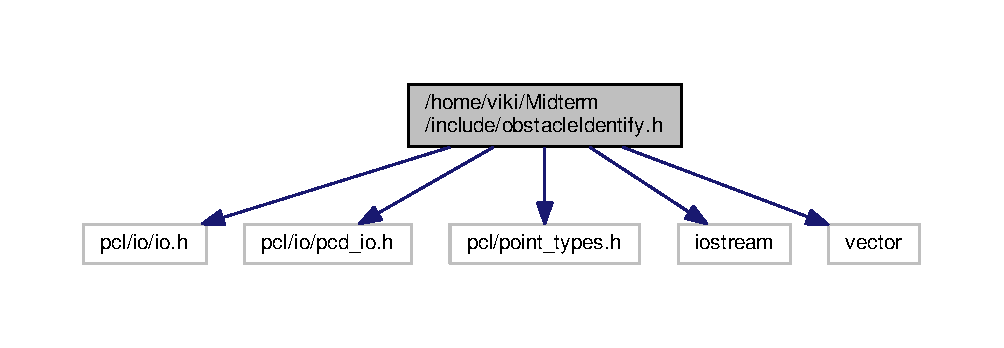
\includegraphics[width=350pt]{obstacleIdentify_8h__incl}
\end{center}
\end{figure}
This graph shows which files directly or indirectly include this file\+:
\nopagebreak
\begin{figure}[H]
\begin{center}
\leavevmode
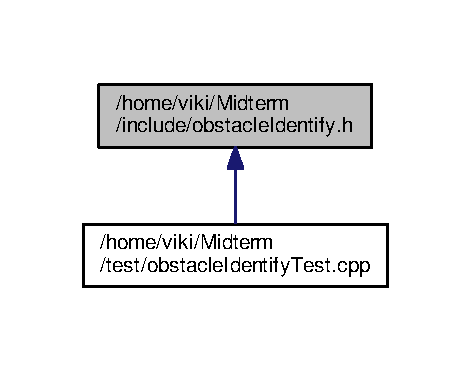
\includegraphics[width=226pt]{obstacleIdentify_8h__dep__incl}
\end{center}
\end{figure}
\subsection*{Classes}
\begin{DoxyCompactItemize}
\item 
class \hyperlink{classobstacleIdentify}{obstacle\+Identify}
\begin{DoxyCompactList}\small\item\em \hyperlink{classobstacleIdentify}{obstacle\+Identify} is an implementation by using point cloud normal to identify an obstacle.
\begin{DoxyItemize}
\item 
\end{DoxyItemize}\end{DoxyCompactList}\end{DoxyCompactItemize}


\subsection{Detailed Description}
header file of an \hyperlink{classobstacleIdentify}{obstacle\+Identify} class. 

This class utilizes point cloud normal to identify an obstacle.

\begin{DoxyAuthor}{Author}
Michael Kam (michael081906) 
\end{DoxyAuthor}
\begin{DoxyRefDesc}{Bug}
\item[\hyperlink{bug__bug000001}{Bug}]No known bugs. \end{DoxyRefDesc}
\begin{DoxyCopyright}{Copyright}
G\+NU Public License. 
\end{DoxyCopyright}

\hypertarget{pclCloudViewer_8h}{}\section{/home/viki/\+Midterm/include/pcl\+Cloud\+Viewer.h File Reference}
\label{pclCloudViewer_8h}\index{/home/viki/\+Midterm/include/pcl\+Cloud\+Viewer.\+h@{/home/viki/\+Midterm/include/pcl\+Cloud\+Viewer.\+h}}


header file of an \hyperlink{classpclCloudViewer}{pcl\+Cloud\+Viewer} class.  


{\ttfamily \#include $<$pcl/visualization/cloud\+\_\+viewer.\+h$>$}\\*
{\ttfamily \#include $<$pcl/io/io.\+h$>$}\\*
{\ttfamily \#include $<$pcl/io/pcd\+\_\+io.\+h$>$}\\*
{\ttfamily \#include $<$pcl/point\+\_\+types.\+h$>$}\\*
{\ttfamily \#include $<$iostream$>$}\\*
Include dependency graph for pcl\+Cloud\+Viewer.\+h\+:
\nopagebreak
\begin{figure}[H]
\begin{center}
\leavevmode
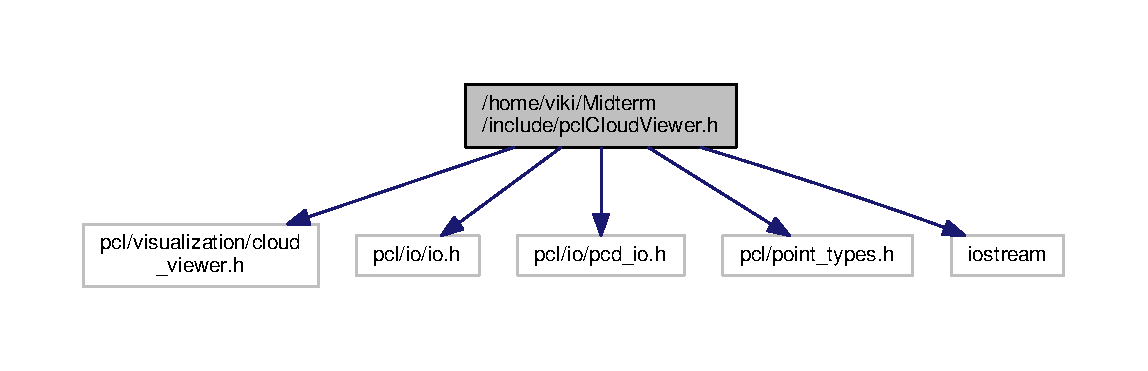
\includegraphics[width=350pt]{pclCloudViewer_8h__incl}
\end{center}
\end{figure}
\subsection*{Classes}
\begin{DoxyCompactItemize}
\item 
class \hyperlink{classpclCloudViewer}{pcl\+Cloud\+Viewer}
\begin{DoxyCompactList}\small\item\em \hyperlink{classpclCloudViewer}{pcl\+Cloud\+Viewer} is an implementation by using pcl visualization to display the point cloud
\begin{DoxyItemize}
\item 
\end{DoxyItemize}\end{DoxyCompactList}\end{DoxyCompactItemize}


\subsection{Detailed Description}
header file of an \hyperlink{classpclCloudViewer}{pcl\+Cloud\+Viewer} class. 

This class utilize pcl visualization to display point cloud.

\begin{DoxyAuthor}{Author}
Michael Kam (michael081906) 
\end{DoxyAuthor}
\begin{DoxyRefDesc}{Bug}
\item[\hyperlink{bug__bug000003}{Bug}]No1 can\textquotesingle{}t not be compile successfully in the test case. \end{DoxyRefDesc}
\begin{DoxyCopyright}{Copyright}
G\+NU Public License. 
\end{DoxyCopyright}

\hypertarget{pclFastTriangular_8h}{}\section{/home/viki/\+Midterm/include/pcl\+Fast\+Triangular.h File Reference}
\label{pclFastTriangular_8h}\index{/home/viki/\+Midterm/include/pcl\+Fast\+Triangular.\+h@{/home/viki/\+Midterm/include/pcl\+Fast\+Triangular.\+h}}


header file of an \hyperlink{classpclFastTriangular}{pcl\+Fast\+Triangular} class.  


{\ttfamily \#include $<$pcl/io/io.\+h$>$}\\*
{\ttfamily \#include $<$pcl/io/pcd\+\_\+io.\+h$>$}\\*
{\ttfamily \#include $<$pcl/point\+\_\+types.\+h$>$}\\*
{\ttfamily \#include $<$pcl/kdtree/kdtree\+\_\+flann.\+h$>$}\\*
{\ttfamily \#include $<$pcl/features/normal\+\_\+3d.\+h$>$}\\*
{\ttfamily \#include $<$pcl/surface/gp3.\+h$>$}\\*
{\ttfamily \#include $<$iostream$>$}\\*
{\ttfamily \#include $<$vector$>$}\\*
{\ttfamily \#include $<$ios$>$}\\*
Include dependency graph for pcl\+Fast\+Triangular.\+h\+:
\nopagebreak
\begin{figure}[H]
\begin{center}
\leavevmode
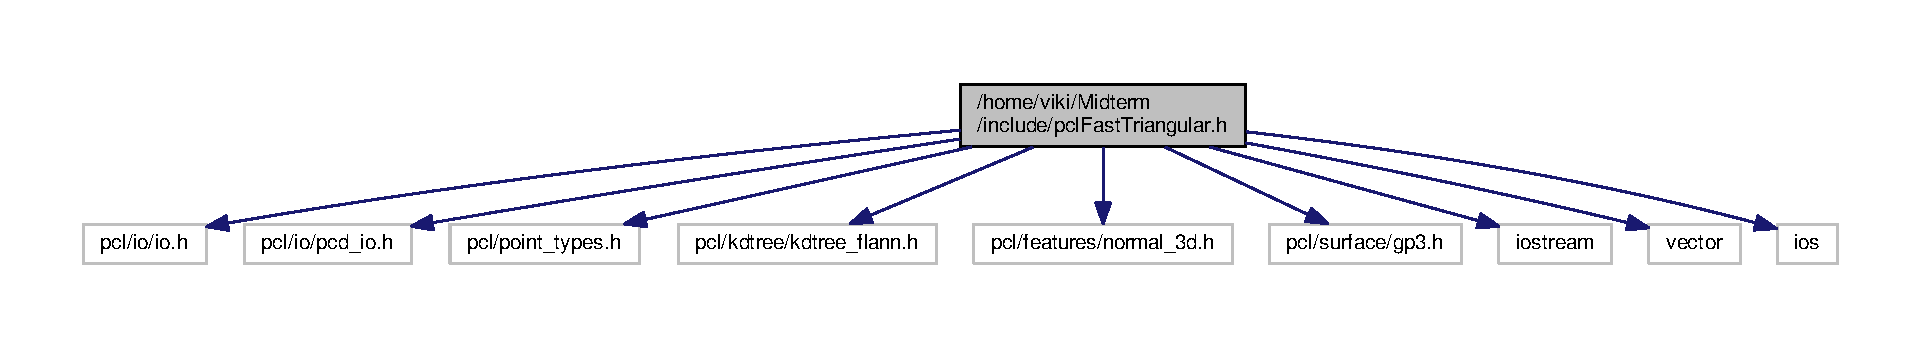
\includegraphics[width=350pt]{pclFastTriangular_8h__incl}
\end{center}
\end{figure}
This graph shows which files directly or indirectly include this file\+:
\nopagebreak
\begin{figure}[H]
\begin{center}
\leavevmode
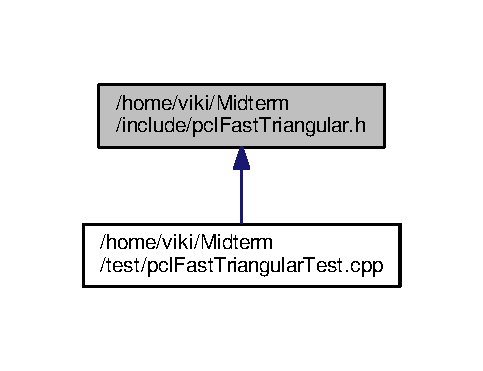
\includegraphics[width=232pt]{pclFastTriangular_8h__dep__incl}
\end{center}
\end{figure}
\subsection*{Classes}
\begin{DoxyCompactItemize}
\item 
class \hyperlink{classpclFastTriangular}{pcl\+Fast\+Triangular}
\begin{DoxyCompactList}\small\item\em \hyperlink{classpclFastTriangular}{pcl\+Fast\+Triangular} is an implementation by using pcl fast\+Triangular method to reconstruct the surface.
\begin{DoxyItemize}
\item 
\end{DoxyItemize}\end{DoxyCompactList}\end{DoxyCompactItemize}


\subsection{Detailed Description}
header file of an \hyperlink{classpclFastTriangular}{pcl\+Fast\+Triangular} class. 

This class utilizes pcl fast\+Triangular method to reconstruct the surface.

\begin{DoxyAuthor}{Author}
Michael Kam (michael081906) 
\end{DoxyAuthor}
\begin{DoxyRefDesc}{Bug}
\item[\hyperlink{bug__bug000005}{Bug}]No known bugs. \end{DoxyRefDesc}
\begin{DoxyCopyright}{Copyright}
G\+NU Public License. 
\end{DoxyCopyright}

\hypertarget{pclIo_8h}{}\section{/home/viki/\+Midterm/include/pcl\+Io.h File Reference}
\label{pclIo_8h}\index{/home/viki/\+Midterm/include/pcl\+Io.\+h@{/home/viki/\+Midterm/include/pcl\+Io.\+h}}


header file of an \hyperlink{classpclIo}{pcl\+Io} class.  


{\ttfamily \#include $<$pcl/io/io.\+h$>$}\\*
{\ttfamily \#include $<$pcl/io/pcd\+\_\+io.\+h$>$}\\*
{\ttfamily \#include $<$pcl/point\+\_\+types.\+h$>$}\\*
{\ttfamily \#include $<$iostream$>$}\\*
{\ttfamily \#include $<$string$>$}\\*
Include dependency graph for pcl\+Io.\+h\+:
\nopagebreak
\begin{figure}[H]
\begin{center}
\leavevmode
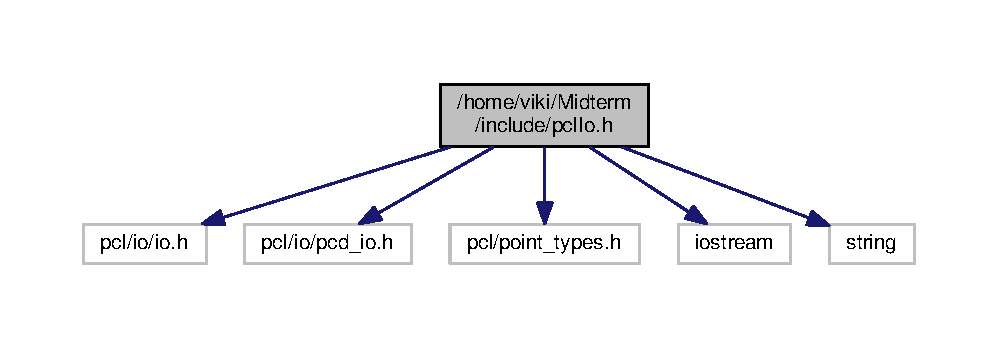
\includegraphics[width=350pt]{pclIo_8h__incl}
\end{center}
\end{figure}
This graph shows which files directly or indirectly include this file\+:
\nopagebreak
\begin{figure}[H]
\begin{center}
\leavevmode
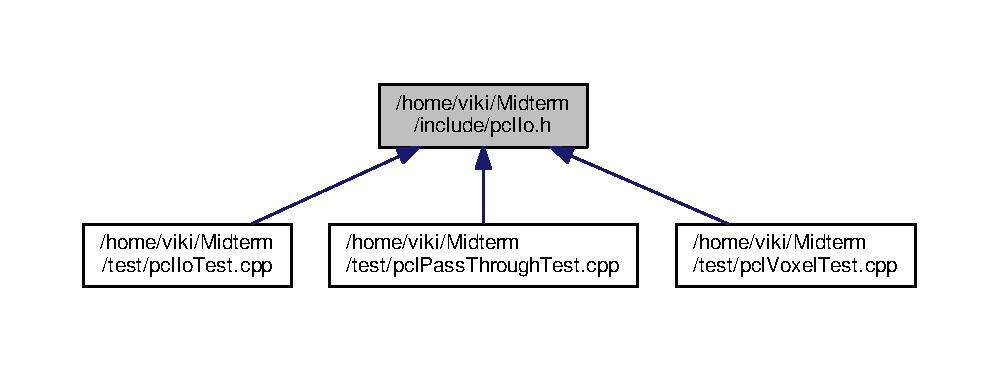
\includegraphics[width=350pt]{pclIo_8h__dep__incl}
\end{center}
\end{figure}
\subsection*{Classes}
\begin{DoxyCompactItemize}
\item 
class \hyperlink{classpclIo}{pcl\+Io}
\begin{DoxyCompactList}\small\item\em \hyperlink{classpclIo}{pcl\+Io} is an implementation by using pcl to load .pcd file from local.
\begin{DoxyItemize}
\item 
\end{DoxyItemize}\end{DoxyCompactList}\end{DoxyCompactItemize}


\subsection{Detailed Description}
header file of an \hyperlink{classpclIo}{pcl\+Io} class. 

This class utilizes pcl to load .pcd file from local.

\begin{DoxyAuthor}{Author}
Michael Kam (michael081906) 
\end{DoxyAuthor}
\begin{DoxyRefDesc}{Bug}
\item[\hyperlink{bug__bug000007}{Bug}]No known bugs. \end{DoxyRefDesc}
\begin{DoxyCopyright}{Copyright}
G\+NU Public License. 
\end{DoxyCopyright}

\hypertarget{pclMlsSmoothing_8h}{}\section{/home/viki/\+Midterm/include/pcl\+Mls\+Smoothing.h File Reference}
\label{pclMlsSmoothing_8h}\index{/home/viki/\+Midterm/include/pcl\+Mls\+Smoothing.\+h@{/home/viki/\+Midterm/include/pcl\+Mls\+Smoothing.\+h}}


header file of an \hyperlink{classpclMlsSmoothing}{pcl\+Mls\+Smoothing} class  


{\ttfamily \#include $<$pcl/io/io.\+h$>$}\\*
{\ttfamily \#include $<$pcl/io/pcd\+\_\+io.\+h$>$}\\*
{\ttfamily \#include $<$pcl/point\+\_\+types.\+h$>$}\\*
{\ttfamily \#include $<$pcl/kdtree/kdtree\+\_\+flann.\+h$>$}\\*
{\ttfamily \#include $<$pcl/surface/mls.\+h$>$}\\*
{\ttfamily \#include $<$iostream$>$}\\*
{\ttfamily \#include $<$vector$>$}\\*
{\ttfamily \#include $<$ios$>$}\\*
Include dependency graph for pcl\+Mls\+Smoothing.\+h\+:
\nopagebreak
\begin{figure}[H]
\begin{center}
\leavevmode
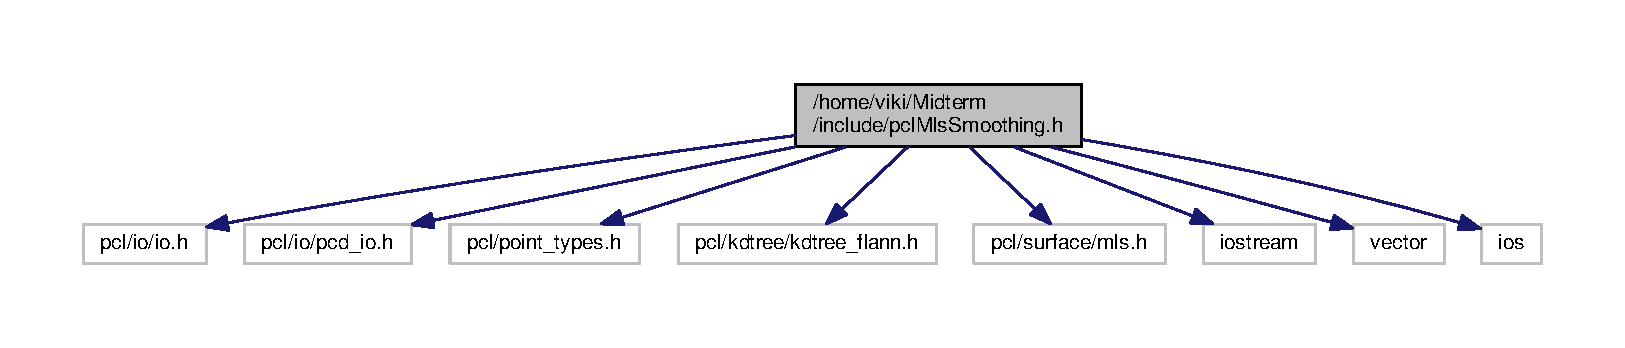
\includegraphics[width=350pt]{pclMlsSmoothing_8h__incl}
\end{center}
\end{figure}
This graph shows which files directly or indirectly include this file\+:
\nopagebreak
\begin{figure}[H]
\begin{center}
\leavevmode
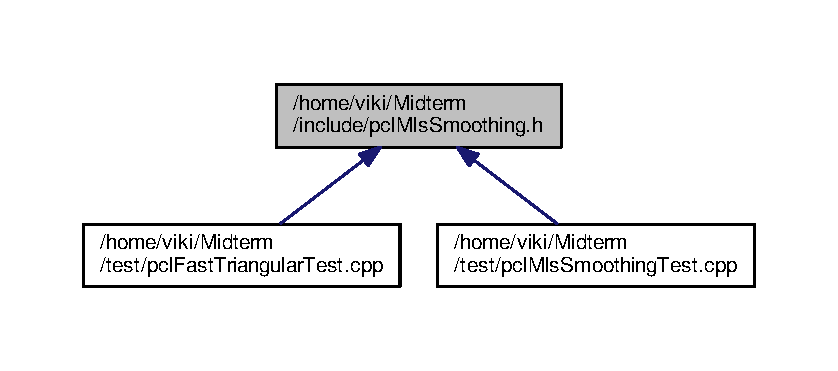
\includegraphics[width=350pt]{pclMlsSmoothing_8h__dep__incl}
\end{center}
\end{figure}
\subsection*{Classes}
\begin{DoxyCompactItemize}
\item 
class \hyperlink{classpclMlsSmoothing}{pcl\+Mls\+Smoothing}
\begin{DoxyCompactList}\small\item\em \hyperlink{classpclMlsSmoothing}{pcl\+Mls\+Smoothing} is an implementation by using moving least square(mls) method to smooth the point cloud among the surface. \end{DoxyCompactList}\end{DoxyCompactItemize}


\subsection{Detailed Description}
header file of an \hyperlink{classpclMlsSmoothing}{pcl\+Mls\+Smoothing} class 

This class utilizes pcl moving least square(mls) method to smooth the point cloud among the surface.

\begin{DoxyAuthor}{Author}
Michael Kam (michael081906) 
\end{DoxyAuthor}
\begin{DoxyRefDesc}{Bug}
\item[\hyperlink{bug__bug000009}{Bug}]No known bugs. \end{DoxyRefDesc}

\hypertarget{pclVoxel_8h}{}\section{/home/viki/\+Midterm/include/pcl\+Voxel.h File Reference}
\label{pclVoxel_8h}\index{/home/viki/\+Midterm/include/pcl\+Voxel.\+h@{/home/viki/\+Midterm/include/pcl\+Voxel.\+h}}


header file of an \hyperlink{classpclVoxel}{pcl\+Voxel} class.  


{\ttfamily \#include $<$pcl/io/io.\+h$>$}\\*
{\ttfamily \#include $<$pcl/io/pcd\+\_\+io.\+h$>$}\\*
{\ttfamily \#include $<$pcl/point\+\_\+types.\+h$>$}\\*
{\ttfamily \#include $<$pcl/filters/voxel\+\_\+grid.\+h$>$}\\*
{\ttfamily \#include $<$vector$>$}\\*
{\ttfamily \#include $<$iostream$>$}\\*
{\ttfamily \#include $<$ios$>$}\\*
Include dependency graph for pcl\+Voxel.\+h\+:
\nopagebreak
\begin{figure}[H]
\begin{center}
\leavevmode
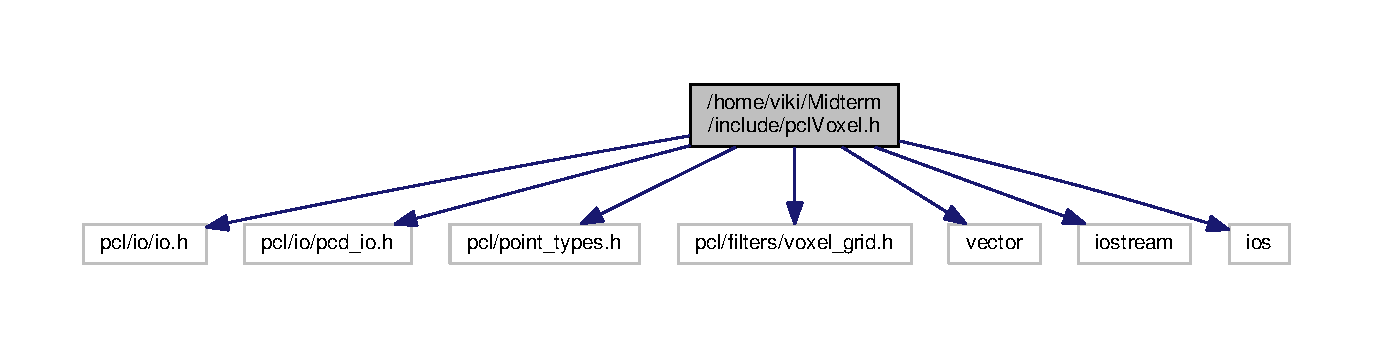
\includegraphics[width=350pt]{pclVoxel_8h__incl}
\end{center}
\end{figure}
This graph shows which files directly or indirectly include this file\+:
\nopagebreak
\begin{figure}[H]
\begin{center}
\leavevmode
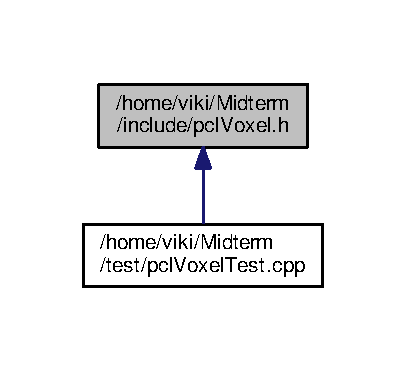
\includegraphics[width=195pt]{pclVoxel_8h__dep__incl}
\end{center}
\end{figure}
\subsection*{Classes}
\begin{DoxyCompactItemize}
\item 
class \hyperlink{classpclVoxel}{pcl\+Voxel}
\begin{DoxyCompactList}\small\item\em \hyperlink{classpclVoxel}{pcl\+Voxel} is an implementation by using pcl voxel\+\_\+grid filter to down sample the point cloud
\begin{DoxyItemize}
\item 
\end{DoxyItemize}\end{DoxyCompactList}\end{DoxyCompactItemize}


\subsection{Detailed Description}
header file of an \hyperlink{classpclVoxel}{pcl\+Voxel} class. 

This class utilize pcl voxel\+\_\+grid filter to down sample the point cloud.

\begin{DoxyAuthor}{Author}
Michael Kam (michael081906) 
\end{DoxyAuthor}
\begin{DoxyRefDesc}{Bug}
\item[\hyperlink{bug__bug000015}{Bug}]No known bugs. \end{DoxyRefDesc}
\begin{DoxyCopyright}{Copyright}
G\+NU Public License. 
\end{DoxyCopyright}

\hypertarget{main_8cpp}{}\section{/home/viki/\+Midterm/test/main.cpp File Reference}
\label{main_8cpp}\index{/home/viki/\+Midterm/test/main.\+cpp@{/home/viki/\+Midterm/test/main.\+cpp}}


main test file of this project.  


{\ttfamily \#include $<$gtest/gtest.\+h$>$}\\*
Include dependency graph for main.\+cpp\+:
\nopagebreak
\begin{figure}[H]
\begin{center}
\leavevmode
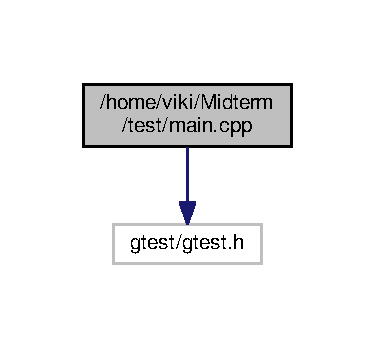
\includegraphics[width=180pt]{main_8cpp__incl}
\end{center}
\end{figure}
\subsection*{Functions}
\begin{DoxyCompactItemize}
\item 
int {\bfseries main} (int argc, char $\ast$$\ast$argv)\hypertarget{main_8cpp_a3c04138a5bfe5d72780bb7e82a18e627}{}\label{main_8cpp_a3c04138a5bfe5d72780bb7e82a18e627}

\end{DoxyCompactItemize}


\subsection{Detailed Description}
main test file of this project. 

The cpp-\/test start entering this file.

\begin{DoxyAuthor}{Author}
Michael Kam (michael081906) 
\end{DoxyAuthor}
\begin{DoxyRefDesc}{Bug}
\item[\hyperlink{bug__bug000017}{Bug}]No known bugs. \end{DoxyRefDesc}
\begin{DoxyCopyright}{Copyright}
G\+NU Public License. 
\end{DoxyCopyright}

\hypertarget{obstacleIdentifyTest_8cpp}{}\section{/home/viki/\+Midterm/test/obstacle\+Identify\+Test.cpp File Reference}
\label{obstacleIdentifyTest_8cpp}\index{/home/viki/\+Midterm/test/obstacle\+Identify\+Test.\+cpp@{/home/viki/\+Midterm/test/obstacle\+Identify\+Test.\+cpp}}


\hyperlink{obstacleIdentifyTest_8cpp}{obstacle\+Identify\+Test.\+cpp} consists of 4 unit test cases that test the \hyperlink{classobstacleIdentify}{obstacle\+Identify} class.  


{\ttfamily \#include $<$gtest/gtest.\+h$>$}\\*
{\ttfamily \#include $<$obstacle\+Identify.\+h$>$}\\*
Include dependency graph for obstacle\+Identify\+Test.\+cpp\+:
\nopagebreak
\begin{figure}[H]
\begin{center}
\leavevmode
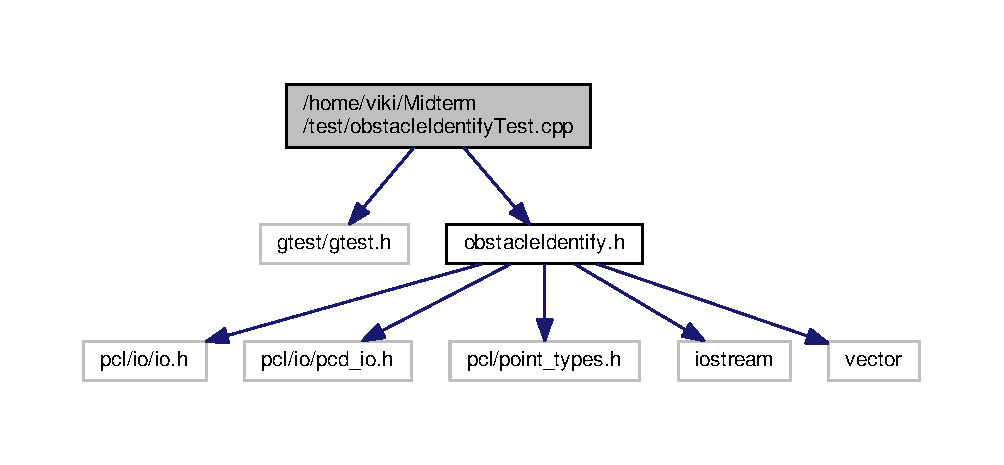
\includegraphics[width=350pt]{obstacleIdentifyTest_8cpp__incl}
\end{center}
\end{figure}
\subsection*{Functions}
\begin{DoxyCompactItemize}
\item 
\hyperlink{obstacleIdentifyTest_8cpp_af116c28e11b80f038d77de4bd6a776b4}{T\+E\+ST} (obstacle\+Identify\+Test, set\+Z\+Height)\hypertarget{obstacleIdentifyTest_8cpp_af116c28e11b80f038d77de4bd6a776b4}{}\label{obstacleIdentifyTest_8cpp_af116c28e11b80f038d77de4bd6a776b4}

\begin{DoxyCompactList}\small\item\em \hyperlink{obstacleIdentifyTest_8cpp_af116c28e11b80f038d77de4bd6a776b4}{T\+E\+S\+T(obstacle\+Identify\+Test, set\+Z\+Height)} will test the set\+Z\+Height() and get\+Z\+Height() method. \end{DoxyCompactList}\item 
\hyperlink{obstacleIdentifyTest_8cpp_a65f93e759aa08ba05802508af4a0909c}{T\+E\+ST} (obstacle\+Identify\+Test, set\+Z\+Normal)\hypertarget{obstacleIdentifyTest_8cpp_a65f93e759aa08ba05802508af4a0909c}{}\label{obstacleIdentifyTest_8cpp_a65f93e759aa08ba05802508af4a0909c}

\begin{DoxyCompactList}\small\item\em \hyperlink{obstacleIdentifyTest_8cpp_a65f93e759aa08ba05802508af4a0909c}{T\+E\+S\+T(obstacle\+Identify\+Test, set\+Z\+Normal)} will test the set\+Normal\+Z() and get\+Normal\+Z() method. \end{DoxyCompactList}\item 
\hyperlink{obstacleIdentifyTest_8cpp_aa8af6d10be97ae6d5279d63300ae3612}{T\+E\+ST} (obstacle\+Identify\+Test, setpcl\+Cloud)\hypertarget{obstacleIdentifyTest_8cpp_aa8af6d10be97ae6d5279d63300ae3612}{}\label{obstacleIdentifyTest_8cpp_aa8af6d10be97ae6d5279d63300ae3612}

\begin{DoxyCompactList}\small\item\em \hyperlink{obstacleIdentifyTest_8cpp_aa8af6d10be97ae6d5279d63300ae3612}{T\+E\+S\+T(obstacle\+Identify\+Test, setpcl\+Cloud)} will test the set\+Input\+Cloud() and get\+Input\+Cloud() method. \end{DoxyCompactList}\item 
\hyperlink{obstacleIdentifyTest_8cpp_a7847d9417fdfc915db6b53334fac42b3}{T\+E\+ST} (obstacle\+Identify\+Test, process)\hypertarget{obstacleIdentifyTest_8cpp_a7847d9417fdfc915db6b53334fac42b3}{}\label{obstacleIdentifyTest_8cpp_a7847d9417fdfc915db6b53334fac42b3}

\begin{DoxyCompactList}\small\item\em \hyperlink{obstacleIdentifyTest_8cpp_a7847d9417fdfc915db6b53334fac42b3}{T\+E\+S\+T(obstacle\+Identify\+Test, process)} will test the process() method. \end{DoxyCompactList}\end{DoxyCompactItemize}


\subsection{Detailed Description}
\hyperlink{obstacleIdentifyTest_8cpp}{obstacle\+Identify\+Test.\+cpp} consists of 4 unit test cases that test the \hyperlink{classobstacleIdentify}{obstacle\+Identify} class. 

\hyperlink{obstacleIdentifyTest_8cpp_af116c28e11b80f038d77de4bd6a776b4}{T\+E\+S\+T(obstacle\+Identify\+Test, set\+Z\+Height)} will test the set\+Z\+Height() and get\+Z\+Height() method. \hyperlink{obstacleIdentifyTest_8cpp_a65f93e759aa08ba05802508af4a0909c}{T\+E\+S\+T(obstacle\+Identify\+Test, set\+Z\+Normal)} will test the set\+Normal\+Z() and get\+Normal\+Z() method. \hyperlink{obstacleIdentifyTest_8cpp_aa8af6d10be97ae6d5279d63300ae3612}{T\+E\+S\+T(obstacle\+Identify\+Test, setpcl\+Cloud)} will test the set\+Input\+Cloud() and get\+Input\+Cloud() method. \hyperlink{obstacleIdentifyTest_8cpp_a7847d9417fdfc915db6b53334fac42b3}{T\+E\+S\+T(obstacle\+Identify\+Test, process)} will test the process() method.

\begin{DoxyAuthor}{Author}
Michael Kam (michael081906) 
\end{DoxyAuthor}
\begin{DoxyRefDesc}{Bug}
\item[\hyperlink{bug__bug000018}{Bug}]No known bugs. \end{DoxyRefDesc}
\begin{DoxyCopyright}{Copyright}
G\+NU Public License. 
\end{DoxyCopyright}

\hypertarget{pclFastTriangularTest_8cpp}{}\section{/home/viki/\+Midterm/test/pcl\+Fast\+Triangular\+Test.cpp File Reference}
\label{pclFastTriangularTest_8cpp}\index{/home/viki/\+Midterm/test/pcl\+Fast\+Triangular\+Test.\+cpp@{/home/viki/\+Midterm/test/pcl\+Fast\+Triangular\+Test.\+cpp}}


\hyperlink{pclFastTriangularTest_8cpp}{pcl\+Fast\+Triangular\+Test.\+cpp} consists of 3 unit test cases that test the \hyperlink{classpclFastTriangular}{pcl\+Fast\+Triangular} class.  


{\ttfamily \#include $<$gtest/gtest.\+h$>$}\\*
{\ttfamily \#include $<$pcl\+Fast\+Triangular.\+h$>$}\\*
{\ttfamily \#include $<$pcl\+Mls\+Smoothing.\+h$>$}\\*
{\ttfamily \#include $<$vector$>$}\\*
Include dependency graph for pcl\+Fast\+Triangular\+Test.\+cpp\+:
\nopagebreak
\begin{figure}[H]
\begin{center}
\leavevmode
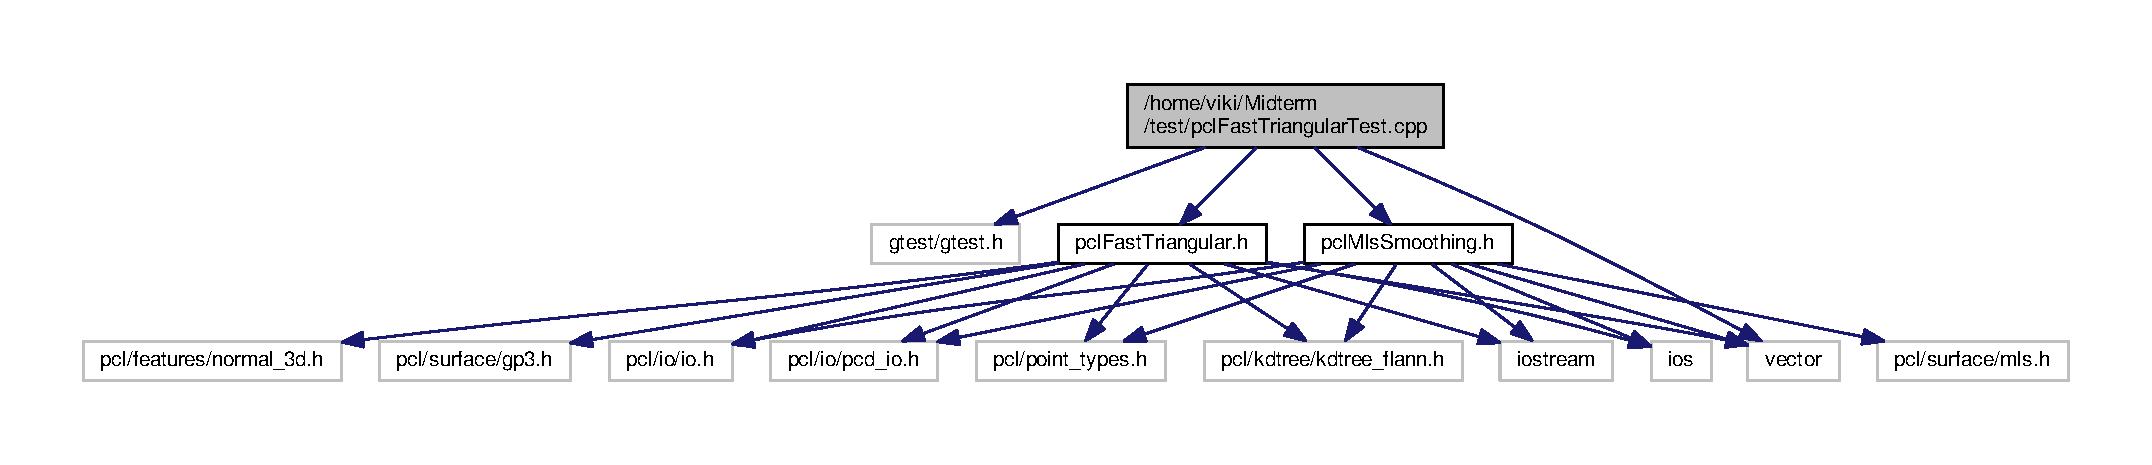
\includegraphics[width=350pt]{pclFastTriangularTest_8cpp__incl}
\end{center}
\end{figure}
\subsection*{Functions}
\begin{DoxyCompactItemize}
\item 
\hyperlink{pclFastTriangularTest_8cpp_a8c383ad3501d8f92cc08103bc7a6f1f5}{T\+E\+ST} (pcl\+Fast\+Triangular\+Test, set\+Radius)\hypertarget{pclFastTriangularTest_8cpp_a8c383ad3501d8f92cc08103bc7a6f1f5}{}\label{pclFastTriangularTest_8cpp_a8c383ad3501d8f92cc08103bc7a6f1f5}

\begin{DoxyCompactList}\small\item\em \hyperlink{pclFastTriangularTest_8cpp_a8c383ad3501d8f92cc08103bc7a6f1f5}{T\+E\+S\+T(pcl\+Fast\+Triangular\+Test, set\+Radius)} will test the set\+Search\+Radius() and get\+Search\+Radius() method. \end{DoxyCompactList}\item 
\hyperlink{pclFastTriangularTest_8cpp_af434c6da69e2cf5de786e4304039d16a}{T\+E\+ST} (pcl\+Fast\+Triangular\+Test, setpcl\+Cloud)\hypertarget{pclFastTriangularTest_8cpp_af434c6da69e2cf5de786e4304039d16a}{}\label{pclFastTriangularTest_8cpp_af434c6da69e2cf5de786e4304039d16a}

\begin{DoxyCompactList}\small\item\em \hyperlink{pclFastTriangularTest_8cpp_af434c6da69e2cf5de786e4304039d16a}{T\+E\+S\+T(pcl\+Fast\+Triangular\+Test, setpcl\+Cloud)} will test the set\+Input\+Cloud() and get\+Input\+Cloud() method. \end{DoxyCompactList}\item 
\hyperlink{pclFastTriangularTest_8cpp_a72dc83c0acb55b59e3dd8bff64ebf8b3}{T\+E\+ST} (pcl\+Fast\+Triangular\+Test, Triangular\+Mesh)\hypertarget{pclFastTriangularTest_8cpp_a72dc83c0acb55b59e3dd8bff64ebf8b3}{}\label{pclFastTriangularTest_8cpp_a72dc83c0acb55b59e3dd8bff64ebf8b3}

\begin{DoxyCompactList}\small\item\em \hyperlink{pclFastTriangularTest_8cpp_a72dc83c0acb55b59e3dd8bff64ebf8b3}{T\+E\+S\+T(pcl\+Fast\+Triangular\+Test, Triangular\+Mesh)} will test the reconctruct() method. \end{DoxyCompactList}\end{DoxyCompactItemize}


\subsection{Detailed Description}
\hyperlink{pclFastTriangularTest_8cpp}{pcl\+Fast\+Triangular\+Test.\+cpp} consists of 3 unit test cases that test the \hyperlink{classpclFastTriangular}{pcl\+Fast\+Triangular} class. 

\hyperlink{pclFastTriangularTest_8cpp_a8c383ad3501d8f92cc08103bc7a6f1f5}{T\+E\+S\+T(pcl\+Fast\+Triangular\+Test, set\+Radius)} will test the set\+Search\+Radius() and get\+Search\+Radius() method. \hyperlink{pclFastTriangularTest_8cpp_af434c6da69e2cf5de786e4304039d16a}{T\+E\+S\+T(pcl\+Fast\+Triangular\+Test, setpcl\+Cloud)} will test the set\+Input\+Cloud() and get\+Input\+Cloud() method. \hyperlink{pclFastTriangularTest_8cpp_a72dc83c0acb55b59e3dd8bff64ebf8b3}{T\+E\+S\+T(pcl\+Fast\+Triangular\+Test, Triangular\+Mesh)} will test the reconctruct() method.

\begin{DoxyAuthor}{Author}
Michael Kam (michael081906) 
\end{DoxyAuthor}
\begin{DoxyRefDesc}{Bug}
\item[\hyperlink{bug__bug000019}{Bug}]No known bugs. \end{DoxyRefDesc}
\begin{DoxyCopyright}{Copyright}
G\+NU Public License. 
\end{DoxyCopyright}

\hypertarget{pclIoTest_8cpp}{}\section{/home/viki/\+Midterm/test/pcl\+Io\+Test.cpp File Reference}
\label{pclIoTest_8cpp}\index{/home/viki/\+Midterm/test/pcl\+Io\+Test.\+cpp@{/home/viki/\+Midterm/test/pcl\+Io\+Test.\+cpp}}


\hyperlink{pclIoTest_8cpp}{pcl\+Io\+Test.\+cpp} consists of 2 unit test cases that test the \hyperlink{classpclIo}{pcl\+Io} class.  


{\ttfamily \#include \char`\"{}pcl\+Io.\+h\char`\"{}}\\*
{\ttfamily \#include $<$pcl/io/pcd\+\_\+io.\+h$>$}\\*
{\ttfamily \#include $<$pcl/point\+\_\+types.\+h$>$}\\*
{\ttfamily \#include $<$gtest/gtest.\+h$>$}\\*
{\ttfamily \#include $<$iostream$>$}\\*
Include dependency graph for pcl\+Io\+Test.\+cpp\+:
\nopagebreak
\begin{figure}[H]
\begin{center}
\leavevmode
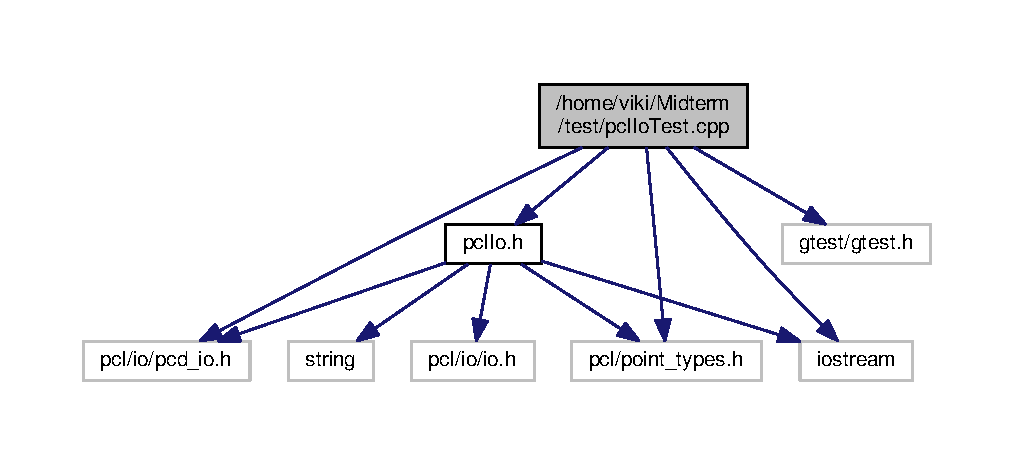
\includegraphics[width=350pt]{pclIoTest_8cpp__incl}
\end{center}
\end{figure}
\subsection*{Functions}
\begin{DoxyCompactItemize}
\item 
\hyperlink{pclIoTest_8cpp_acadc143b86b8db1747d4dfd44ae475e3}{T\+E\+ST} (pcl\+Io\+Test, load\+P\+C\+Dfile\+Must\+Fail)\hypertarget{pclIoTest_8cpp_acadc143b86b8db1747d4dfd44ae475e3}{}\label{pclIoTest_8cpp_acadc143b86b8db1747d4dfd44ae475e3}

\begin{DoxyCompactList}\small\item\em \hyperlink{pclIoTest_8cpp_acadc143b86b8db1747d4dfd44ae475e3}{T\+E\+S\+T(pcl\+Io\+Test, load\+P\+C\+Dfile\+Must\+Fail)} will test the read\+P\+C\+Dfile() method. \end{DoxyCompactList}\item 
\hyperlink{pclIoTest_8cpp_aaf03e3af6aa987fa78da874364eaf931}{T\+E\+ST} (pcl\+Io\+Test, load\+P\+C\+Dfile\+Show\+Result)\hypertarget{pclIoTest_8cpp_aaf03e3af6aa987fa78da874364eaf931}{}\label{pclIoTest_8cpp_aaf03e3af6aa987fa78da874364eaf931}

\begin{DoxyCompactList}\small\item\em \hyperlink{pclIoTest_8cpp_aaf03e3af6aa987fa78da874364eaf931}{T\+E\+S\+T(pcl\+Io\+Test, load\+P\+C\+Dfile\+Show\+Result)} will test the get\+Point\+Cloud() method. \end{DoxyCompactList}\end{DoxyCompactItemize}


\subsection{Detailed Description}
\hyperlink{pclIoTest_8cpp}{pcl\+Io\+Test.\+cpp} consists of 2 unit test cases that test the \hyperlink{classpclIo}{pcl\+Io} class. 

\hyperlink{pclIoTest_8cpp_acadc143b86b8db1747d4dfd44ae475e3}{T\+E\+S\+T(pcl\+Io\+Test, load\+P\+C\+Dfile\+Must\+Fail)} will test the read\+P\+C\+Dfile() method. \hyperlink{pclIoTest_8cpp_aaf03e3af6aa987fa78da874364eaf931}{T\+E\+S\+T(pcl\+Io\+Test, load\+P\+C\+Dfile\+Show\+Result)} will test the get\+Point\+Cloud() method.

\begin{DoxyAuthor}{Author}
Michael Kam (michael081906) 
\end{DoxyAuthor}
\begin{DoxyRefDesc}{Bug}
\item[\hyperlink{bug__bug000020}{Bug}]No known bugs. \end{DoxyRefDesc}
\begin{DoxyCopyright}{Copyright}
G\+NU Public License. 
\end{DoxyCopyright}

\hypertarget{pclMlsSmoothingTest_8cpp}{}\section{/home/viki/\+Midterm/test/pcl\+Mls\+Smoothing\+Test.cpp File Reference}
\label{pclMlsSmoothingTest_8cpp}\index{/home/viki/\+Midterm/test/pcl\+Mls\+Smoothing\+Test.\+cpp@{/home/viki/\+Midterm/test/pcl\+Mls\+Smoothing\+Test.\+cpp}}


\hyperlink{pclMlsSmoothingTest_8cpp}{pcl\+Mls\+Smoothing\+Test.\+cpp} consists of 3 unit test cases that test the \hyperlink{classpclMlsSmoothing}{pcl\+Mls\+Smoothing} class.  


{\ttfamily \#include $<$gtest/gtest.\+h$>$}\\*
{\ttfamily \#include $<$pcl\+Mls\+Smoothing.\+h$>$}\\*
Include dependency graph for pcl\+Mls\+Smoothing\+Test.\+cpp\+:
\nopagebreak
\begin{figure}[H]
\begin{center}
\leavevmode
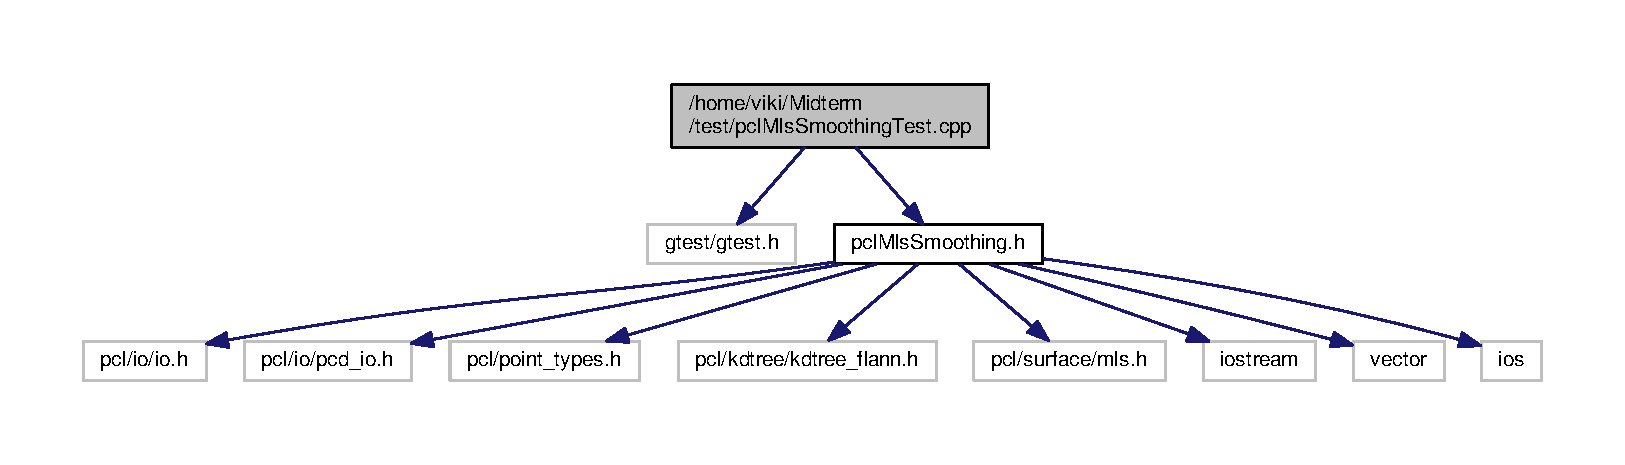
\includegraphics[width=350pt]{pclMlsSmoothingTest_8cpp__incl}
\end{center}
\end{figure}
\subsection*{Functions}
\begin{DoxyCompactItemize}
\item 
\hyperlink{pclMlsSmoothingTest_8cpp_a108228ab9f6b7dc193551c5025b26b69}{T\+E\+ST} (pcl\+Mls\+Smoothing\+Test, set\+Radius)\hypertarget{pclMlsSmoothingTest_8cpp_a108228ab9f6b7dc193551c5025b26b69}{}\label{pclMlsSmoothingTest_8cpp_a108228ab9f6b7dc193551c5025b26b69}

\begin{DoxyCompactList}\small\item\em \hyperlink{pclMlsSmoothingTest_8cpp_a108228ab9f6b7dc193551c5025b26b69}{T\+E\+S\+T(pcl\+Mls\+Smoothing\+Test, set\+Radius)} will test the set\+Search\+Radius() and get\+Search\+Radius() method. \end{DoxyCompactList}\item 
\hyperlink{pclMlsSmoothingTest_8cpp_a0f0895afe16f423a9b57b8da0f4a2749}{T\+E\+ST} (pcl\+Mls\+Smoothing\+Test, setpcl\+Cloud)\hypertarget{pclMlsSmoothingTest_8cpp_a0f0895afe16f423a9b57b8da0f4a2749}{}\label{pclMlsSmoothingTest_8cpp_a0f0895afe16f423a9b57b8da0f4a2749}

\begin{DoxyCompactList}\small\item\em \hyperlink{pclMlsSmoothingTest_8cpp_a0f0895afe16f423a9b57b8da0f4a2749}{T\+E\+S\+T(pcl\+Mls\+Smoothing\+Test, setpcl\+Cloud)} will test the get\+Input\+Cloud() and set\+Input\+Cloud() method. \end{DoxyCompactList}\item 
\hyperlink{pclMlsSmoothingTest_8cpp_a2438d2c1b948a4136db5fcb288f9ca87}{T\+E\+ST} (pcl\+Mls\+Smoothing\+Test, Mls\+Filtering)\hypertarget{pclMlsSmoothingTest_8cpp_a2438d2c1b948a4136db5fcb288f9ca87}{}\label{pclMlsSmoothingTest_8cpp_a2438d2c1b948a4136db5fcb288f9ca87}

\begin{DoxyCompactList}\small\item\em \hyperlink{pclMlsSmoothingTest_8cpp_a2438d2c1b948a4136db5fcb288f9ca87}{T\+E\+S\+T(pcl\+Mls\+Smoothing\+Test, Mls\+Filtering)} will test the mls\+Process() \end{DoxyCompactList}\end{DoxyCompactItemize}


\subsection{Detailed Description}
\hyperlink{pclMlsSmoothingTest_8cpp}{pcl\+Mls\+Smoothing\+Test.\+cpp} consists of 3 unit test cases that test the \hyperlink{classpclMlsSmoothing}{pcl\+Mls\+Smoothing} class. 

\hyperlink{pclMlsSmoothingTest_8cpp_a108228ab9f6b7dc193551c5025b26b69}{T\+E\+S\+T(pcl\+Mls\+Smoothing\+Test, set\+Radius)} will test the set\+Search\+Radius() and get\+Search\+Radius() method. \hyperlink{pclMlsSmoothingTest_8cpp_a0f0895afe16f423a9b57b8da0f4a2749}{T\+E\+S\+T(pcl\+Mls\+Smoothing\+Test, setpcl\+Cloud)} will test the get\+Input\+Cloud() and set\+Input\+Cloud() method. \hyperlink{pclMlsSmoothingTest_8cpp_a2438d2c1b948a4136db5fcb288f9ca87}{T\+E\+S\+T(pcl\+Mls\+Smoothing\+Test, Mls\+Filtering)} will test the mls\+Process().

\begin{DoxyAuthor}{Author}
Michael Kam (michael081906) 
\end{DoxyAuthor}
\begin{DoxyRefDesc}{Bug}
\item[\hyperlink{bug__bug000021}{Bug}]No known bugs. \end{DoxyRefDesc}
\begin{DoxyCopyright}{Copyright}
G\+NU Public License. 
\end{DoxyCopyright}

\hypertarget{pclPassThroughTest_8cpp}{}\section{/home/viki/\+Midterm/test/pcl\+Pass\+Through\+Test.cpp File Reference}
\label{pclPassThroughTest_8cpp}\index{/home/viki/\+Midterm/test/pcl\+Pass\+Through\+Test.\+cpp@{/home/viki/\+Midterm/test/pcl\+Pass\+Through\+Test.\+cpp}}


\hyperlink{pclPassThroughTest_8cpp}{pcl\+Pass\+Through\+Test.\+cpp} consists of 2 unit test cases that test the \hyperlink{classpclPassThrough}{pcl\+Pass\+Through} class.  


{\ttfamily \#include \char`\"{}pcl\+Io.\+h\char`\"{}}\\*
{\ttfamily \#include \char`\"{}pcl\+Pass\+Through.\+h\char`\"{}}\\*
{\ttfamily \#include $<$gtest/gtest.\+h$>$}\\*
{\ttfamily \#include $<$pcl/io/pcd\+\_\+io.\+h$>$}\\*
{\ttfamily \#include $<$pcl/point\+\_\+types.\+h$>$}\\*
{\ttfamily \#include $<$vector$>$}\\*
{\ttfamily \#include $<$iostream$>$}\\*
Include dependency graph for pcl\+Pass\+Through\+Test.\+cpp\+:
\nopagebreak
\begin{figure}[H]
\begin{center}
\leavevmode
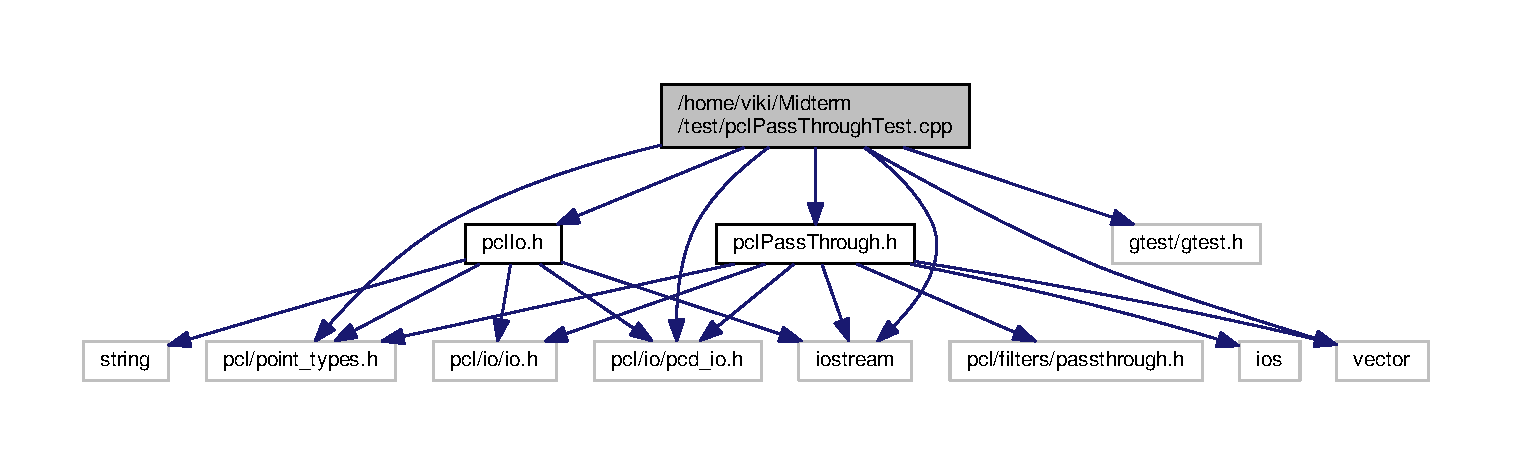
\includegraphics[width=350pt]{pclPassThroughTest_8cpp__incl}
\end{center}
\end{figure}
\subsection*{Functions}
\begin{DoxyCompactItemize}
\item 
\hyperlink{pclPassThroughTest_8cpp_a17ba3ae7544ab54598271bb424069d19}{T\+E\+ST} (pcl\+Pass\+Through\+Test, set\+Limit\+Value)\hypertarget{pclPassThroughTest_8cpp_a17ba3ae7544ab54598271bb424069d19}{}\label{pclPassThroughTest_8cpp_a17ba3ae7544ab54598271bb424069d19}

\begin{DoxyCompactList}\small\item\em \hyperlink{pclPassThroughTest_8cpp_a17ba3ae7544ab54598271bb424069d19}{T\+E\+S\+T(pcl\+Pass\+Through\+Test, set\+Limit\+Value)} will test the set\+Filter\+Xlimit() ,set\+Filter\+Ylimit, set\+Filter\+Zlimit(), and get\+Filter\+Limit() method. \end{DoxyCompactList}\item 
\hyperlink{pclPassThroughTest_8cpp_a3288389cf8648f9cd5967e14765849a1}{T\+E\+ST} (pcl\+Pass\+Through\+Test, Pass\+Through\+Filtered)\hypertarget{pclPassThroughTest_8cpp_a3288389cf8648f9cd5967e14765849a1}{}\label{pclPassThroughTest_8cpp_a3288389cf8648f9cd5967e14765849a1}

\begin{DoxyCompactList}\small\item\em \hyperlink{pclPassThroughTest_8cpp_a3288389cf8648f9cd5967e14765849a1}{T\+E\+S\+T(pcl\+Pass\+Through\+Test, Pass\+Through\+Filtered)} will test the filter\+Process() method. \end{DoxyCompactList}\end{DoxyCompactItemize}


\subsection{Detailed Description}
\hyperlink{pclPassThroughTest_8cpp}{pcl\+Pass\+Through\+Test.\+cpp} consists of 2 unit test cases that test the \hyperlink{classpclPassThrough}{pcl\+Pass\+Through} class. 

\hyperlink{pclPassThroughTest_8cpp_a17ba3ae7544ab54598271bb424069d19}{T\+E\+S\+T(pcl\+Pass\+Through\+Test, set\+Limit\+Value)} will test the set\+Filter\+Xlimit() ,set\+Filter\+Ylimit, set\+Filter\+Zlimit(), and get\+Filter\+Limit() method. \hyperlink{pclPassThroughTest_8cpp_a3288389cf8648f9cd5967e14765849a1}{T\+E\+S\+T(pcl\+Pass\+Through\+Test, Pass\+Through\+Filtered)} will test the filter\+Process() method.

\begin{DoxyAuthor}{Author}
Michael Kam (michael081906) 
\end{DoxyAuthor}
\begin{DoxyRefDesc}{Bug}
\item[\hyperlink{bug__bug000022}{Bug}]No known bugs. \end{DoxyRefDesc}
\begin{DoxyCopyright}{Copyright}
G\+NU Public License. 
\end{DoxyCopyright}

\hypertarget{pclStatisticalOutlierRemovalTest_8cpp}{}\section{/home/viki/\+Midterm/test/pcl\+Statistical\+Outlier\+Removal\+Test.cpp File Reference}
\label{pclStatisticalOutlierRemovalTest_8cpp}\index{/home/viki/\+Midterm/test/pcl\+Statistical\+Outlier\+Removal\+Test.\+cpp@{/home/viki/\+Midterm/test/pcl\+Statistical\+Outlier\+Removal\+Test.\+cpp}}


\hyperlink{pclStatisticalOutlierRemovalTest_8cpp}{pcl\+Statistical\+Outlier\+Removal\+Test.\+cpp} consists of 3 unit test cases that test the pcl\+Statistical\+Outlier\+Removal class.  


{\ttfamily \#include $<$gtest/gtest.\+h$>$}\\*
{\ttfamily \#include $<$pcl/point\+\_\+types.\+h$>$}\\*
{\ttfamily \#include \char`\"{}pcl\+Statistical\+Outlier\+Removal.\+h\char`\"{}}\\*
{\ttfamily \#include $<$iostream$>$}\\*
{\ttfamily \#include $<$vector$>$}\\*
Include dependency graph for pcl\+Statistical\+Outlier\+Removal\+Test.\+cpp\+:
\nopagebreak
\begin{figure}[H]
\begin{center}
\leavevmode
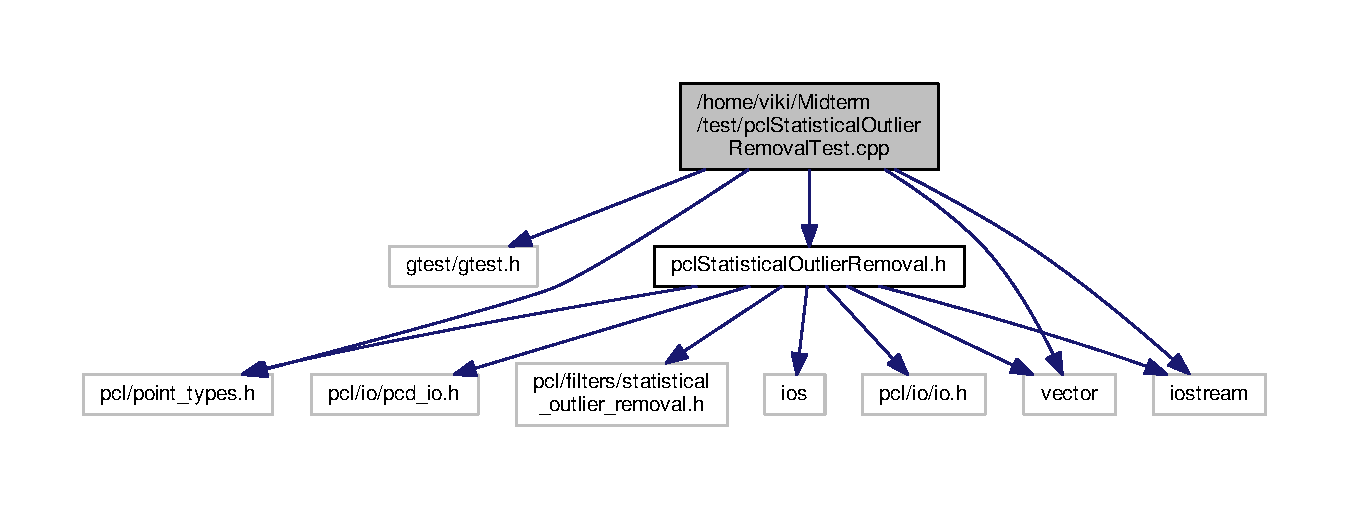
\includegraphics[width=350pt]{pclStatisticalOutlierRemovalTest_8cpp__incl}
\end{center}
\end{figure}
\subsection*{Functions}
\begin{DoxyCompactItemize}
\item 
\hyperlink{pclStatisticalOutlierRemovalTest_8cpp_a7440b4567b31e478a4e0db15713a13df}{T\+E\+ST} (pcl\+Statistical\+Outlier\+Removal\+Test, Set\+Meank\+And\+Thresh)
\item 
\hyperlink{pclStatisticalOutlierRemovalTest_8cpp_ab4412c4c90dfee3682f0cfacb6f02226}{T\+E\+ST} (pcl\+Statistical\+Outlier\+Removal\+Test, Set\+Point\+Cloud)\hypertarget{pclStatisticalOutlierRemovalTest_8cpp_ab4412c4c90dfee3682f0cfacb6f02226}{}\label{pclStatisticalOutlierRemovalTest_8cpp_ab4412c4c90dfee3682f0cfacb6f02226}

\begin{DoxyCompactList}\small\item\em T\+E\+ST(pcl\+Statistical\+Outlier\+Removal\+Test, Set\+Point\+Cloud) will test the get\+Input\+Cloud() and set\+Input\+Cloud() method. \end{DoxyCompactList}\item 
\hyperlink{pclStatisticalOutlierRemovalTest_8cpp_a4bd86cf4614402db58c7e3da6340f15a}{T\+E\+ST} (pcl\+Statistical\+Outlier\+Removal\+Test, S\+O\+R\+Filter\+Test)\hypertarget{pclStatisticalOutlierRemovalTest_8cpp_a4bd86cf4614402db58c7e3da6340f15a}{}\label{pclStatisticalOutlierRemovalTest_8cpp_a4bd86cf4614402db58c7e3da6340f15a}

\begin{DoxyCompactList}\small\item\em \hyperlink{pclStatisticalOutlierRemovalTest_8cpp_a4bd86cf4614402db58c7e3da6340f15a}{T\+E\+S\+T(pcl\+Statistical\+Outlier\+Removal\+Test, S\+O\+R\+Filter\+Test)} will test the filter\+Process() method. \end{DoxyCompactList}\end{DoxyCompactItemize}


\subsection{Detailed Description}
\hyperlink{pclStatisticalOutlierRemovalTest_8cpp}{pcl\+Statistical\+Outlier\+Removal\+Test.\+cpp} consists of 3 unit test cases that test the pcl\+Statistical\+Outlier\+Removal class. 

\hyperlink{pclStatisticalOutlierRemovalTest_8cpp_a7440b4567b31e478a4e0db15713a13df}{T\+E\+S\+T(pcl\+Statistical\+Outlier\+Removal\+Test, Set\+Meank\+And\+Thresh)} will test the get\+Mean\+K(), set\+Stddev\+Mul\+Thresh(), set\+Mean\+K(), and get\+Stddev\+Mul\+Thresh() method. \hyperlink{pclStatisticalOutlierRemovalTest_8cpp_ab4412c4c90dfee3682f0cfacb6f02226}{T\+E\+S\+T(pcl\+Statistical\+Outlier\+Removal\+Test, Set\+Point\+Cloud)} will test the get\+Input\+Cloud() and set\+Input\+Cloud() method. \hyperlink{pclStatisticalOutlierRemovalTest_8cpp_a4bd86cf4614402db58c7e3da6340f15a}{T\+E\+S\+T(pcl\+Statistical\+Outlier\+Removal\+Test, S\+O\+R\+Filter\+Test)} will test the filter\+Process() method.

\begin{DoxyAuthor}{Author}
Michael Kam (michael081906) 
\end{DoxyAuthor}
\begin{DoxyRefDesc}{Bug}
\item[\hyperlink{bug__bug000023}{Bug}]No known bugs. \end{DoxyRefDesc}
\begin{DoxyCopyright}{Copyright}
G\+NU Public License. 
\end{DoxyCopyright}


\subsection{Function Documentation}
\index{pcl\+Statistical\+Outlier\+Removal\+Test.\+cpp@{pcl\+Statistical\+Outlier\+Removal\+Test.\+cpp}!T\+E\+ST@{T\+E\+ST}}
\index{T\+E\+ST@{T\+E\+ST}!pcl\+Statistical\+Outlier\+Removal\+Test.\+cpp@{pcl\+Statistical\+Outlier\+Removal\+Test.\+cpp}}
\subsubsection[{\texorpdfstring{T\+E\+S\+T(pcl\+Statistical\+Outlier\+Removal\+Test, Set\+Meank\+And\+Thresh)}{TEST(pclStatisticalOutlierRemovalTest, SetMeankAndThresh)}}]{\setlength{\rightskip}{0pt plus 5cm}T\+E\+ST (
\begin{DoxyParamCaption}
\item[{pcl\+Statistical\+Outlier\+Removal\+Test}]{, }
\item[{Set\+Meank\+And\+Thresh}]{}
\end{DoxyParamCaption}
)}\hypertarget{pclStatisticalOutlierRemovalTest_8cpp_a7440b4567b31e478a4e0db15713a13df}{}\label{pclStatisticalOutlierRemovalTest_8cpp_a7440b4567b31e478a4e0db15713a13df}
@ brief T\+E\+ST(pcl\+Statistical\+Outlier\+Removal\+Test, Set\+Meank\+And\+Thresh) will test the get\+Mean\+K(), set\+Stddev\+Mul\+Thresh(), set\+Mean\+K(), and get\+Stddev\+Mul\+Thresh() method. 
\hypertarget{pclVoxelTest_8cpp}{}\section{/home/viki/\+Midterm/test/pcl\+Voxel\+Test.cpp File Reference}
\label{pclVoxelTest_8cpp}\index{/home/viki/\+Midterm/test/pcl\+Voxel\+Test.\+cpp@{/home/viki/\+Midterm/test/pcl\+Voxel\+Test.\+cpp}}


\hyperlink{pclVoxelTest_8cpp}{pcl\+Voxel\+Test.\+cpp} consists of 3 unit test cases that test the \hyperlink{classpclVoxel}{pcl\+Voxel} class.  


{\ttfamily \#include \char`\"{}pcl\+Voxel.\+h\char`\"{}}\\*
{\ttfamily \#include \char`\"{}pcl\+Io.\+h\char`\"{}}\\*
{\ttfamily \#include $<$gtest/gtest.\+h$>$}\\*
{\ttfamily \#include $<$pcl/io/pcd\+\_\+io.\+h$>$}\\*
{\ttfamily \#include $<$pcl/point\+\_\+types.\+h$>$}\\*
{\ttfamily \#include $<$iostream$>$}\\*
{\ttfamily \#include $<$vector$>$}\\*
Include dependency graph for pcl\+Voxel\+Test.\+cpp\+:
\nopagebreak
\begin{figure}[H]
\begin{center}
\leavevmode
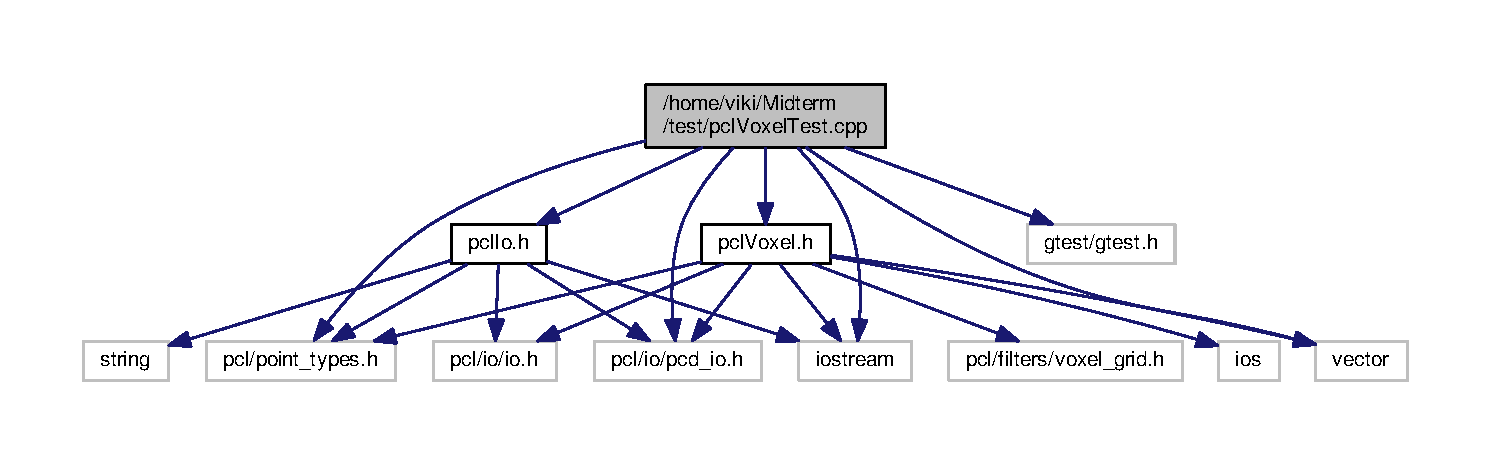
\includegraphics[width=350pt]{pclVoxelTest_8cpp__incl}
\end{center}
\end{figure}
\subsection*{Functions}
\begin{DoxyCompactItemize}
\item 
\hyperlink{pclVoxelTest_8cpp_ab975b9c05d07fcea10cd0d3a9ce5ab3e}{T\+E\+ST} (pcl\+Voxel\+Test, set\+Leaf\+Value)\hypertarget{pclVoxelTest_8cpp_ab975b9c05d07fcea10cd0d3a9ce5ab3e}{}\label{pclVoxelTest_8cpp_ab975b9c05d07fcea10cd0d3a9ce5ab3e}

\begin{DoxyCompactList}\small\item\em \hyperlink{pclVoxelTest_8cpp_ab975b9c05d07fcea10cd0d3a9ce5ab3e}{T\+E\+S\+T(pcl\+Voxel\+Test, set\+Leaf\+Value)} will test the set\+Leaf\+Size() and get\+Leaf\+Size() method. \end{DoxyCompactList}\item 
\hyperlink{pclVoxelTest_8cpp_a1dccf2e8837d1aa845509b9985792722}{T\+E\+ST} (pcl\+Voxel\+Test, point\+Cloud\+Down\+Sampleing)\hypertarget{pclVoxelTest_8cpp_a1dccf2e8837d1aa845509b9985792722}{}\label{pclVoxelTest_8cpp_a1dccf2e8837d1aa845509b9985792722}

\begin{DoxyCompactList}\small\item\em \hyperlink{pclVoxelTest_8cpp_a1dccf2e8837d1aa845509b9985792722}{T\+E\+S\+T(pcl\+Voxel\+Test, point\+Cloud\+Down\+Sampleing)} will test the filter\+Process() method. \end{DoxyCompactList}\item 
\hyperlink{pclVoxelTest_8cpp_a8f1ee4768a36f1296e75ac0b7c4b6b3d}{T\+E\+ST} (pcl\+Voxel\+Test, setpcl\+Cloud)\hypertarget{pclVoxelTest_8cpp_a8f1ee4768a36f1296e75ac0b7c4b6b3d}{}\label{pclVoxelTest_8cpp_a8f1ee4768a36f1296e75ac0b7c4b6b3d}

\begin{DoxyCompactList}\small\item\em \hyperlink{pclVoxelTest_8cpp_a8f1ee4768a36f1296e75ac0b7c4b6b3d}{T\+E\+S\+T(pcl\+Voxel\+Test, setpcl\+Cloud)} will test the get\+Input\+Cloud() and set\+Input\+Cloud() method. \end{DoxyCompactList}\end{DoxyCompactItemize}


\subsection{Detailed Description}
\hyperlink{pclVoxelTest_8cpp}{pcl\+Voxel\+Test.\+cpp} consists of 3 unit test cases that test the \hyperlink{classpclVoxel}{pcl\+Voxel} class. 

\hyperlink{pclVoxelTest_8cpp_ab975b9c05d07fcea10cd0d3a9ce5ab3e}{T\+E\+S\+T(pcl\+Voxel\+Test, set\+Leaf\+Value)} will test the set\+Leaf\+Size() and get\+Leaf\+Size() method. \hyperlink{pclVoxelTest_8cpp_a1dccf2e8837d1aa845509b9985792722}{T\+E\+S\+T(pcl\+Voxel\+Test, point\+Cloud\+Down\+Sampleing)} will test the filter\+Process() method. \hyperlink{pclVoxelTest_8cpp_a8f1ee4768a36f1296e75ac0b7c4b6b3d}{T\+E\+S\+T(pcl\+Voxel\+Test, setpcl\+Cloud)} will test the get\+Input\+Cloud() and set\+Input\+Cloud() method.

\begin{DoxyAuthor}{Author}
Michael Kam (michael081906) 
\end{DoxyAuthor}
\begin{DoxyRefDesc}{Bug}
\item[\hyperlink{bug__bug000024}{Bug}]No known bugs. \end{DoxyRefDesc}
\begin{DoxyCopyright}{Copyright}
G\+NU Public License. 
\end{DoxyCopyright}

%--- End generated contents ---

% Index
\backmatter
\newpage
\phantomsection
\clearemptydoublepage
\addcontentsline{toc}{chapter}{Index}
\printindex

\end{document}
